%%%%%%%%%%%%%%%%%%%%%%%%%%%%%%%%%%%%%%%%%
% Stylish Article
% LaTeX Template
% Version 2.1 (1/10/15)
%
% This template has been downloaded from:
% http://www.LaTeXTemplates.com
%
% Original author:
% Mathias Legrand (legrand.mathias@gmail.com) 
% With extensive modifications by:
% Vel (vel@latextemplates.com)
%
% License:
% CC BY-NC-SA 3.0 (http://creativecommons.org/licenses/by-nc-sa/3.0/)
%
%%%%%%%%%%%%%%%%%%%%%%%%%%%%%%%%%%%%%%%%%

%----------------------------------------------------------------------------------------
%	PACKAGES AND OTHER DOCUMENT CONFIGURATIONS
%----------------------------------------------------------------------------------------

\documentclass[fleqn,10pt]{SelfArx} % Document font size and equations flushed left

\usepackage[english]{babel} % Specify a different language here - english by default

\usepackage{lipsum} % Required to insert dummy text. To be removed otherwise

%----------------------------------------------------------------------------------------
%	COLUMNS
%----------------------------------------------------------------------------------------

\setlength{\columnsep}{0.55cm} % Distance between the two columns of text
\setlength{\fboxrule}{0.75pt} % Width of the border around the abstract

%----------------------------------------------------------------------------------------
%	COLORS
%----------------------------------------------------------------------------------------

\definecolor{color1}{RGB}{0,0,90} % Color of the article title and sections
\definecolor{color2}{RGB}{0,20,20} % Color of the boxes behind the abstract and headings

%----------------------------------------------------------------------------------------
%	HYPERLINKS
%----------------------------------------------------------------------------------------

\usepackage{hyperref} % Required for hyperlinks
\hypersetup{hidelinks,colorlinks,breaklinks=true,urlcolor=color2,citecolor=color1,linkcolor=color1,bookmarksopen=false,pdftitle={Title},pdfauthor={Author}}

%----------------------------------------------------------------------------------------
%	ARTICLE INFORMATION
%----------------------------------------------------------------------------------------

\JournalInfo{Journal of Praba's curiosity , Vol. I, No. 1, 1-5, 2017} % Journal information
\Archive{@prabasiva} % Additional notes (e.g. copyright, DOI, review/research article)

\PaperTitle{Dynamics of Amazon's diversified business model} % Article title

%\Authors{Praba Siva\textsuperscript{1}* } % Authors
%\affiliation{\textsuperscript{1}\textit{Department of Applied Mathematics, University of Michigan, Dearborn, Michigan}} % Author affiliation
%\affiliation{*\textbf{Corresponding author}: praba@umich.edu} % Corresponding author
\Authors{Praba Siva\textsuperscript{1}* } % Authors
\affiliation{\textsuperscript{1}\textit{Department of Mathematics \& Statistics , University of Michigan, Dearborn, MI}} % Author affiliation
\affiliation{*\textbf{Corresponding author}: praba@umich.edu} % Corresponding author

\Keywords{Amazon --- Dynamial Systems --- Cloud Computing --- Business Strategy --- Competitive analysis --- Game Theory --- Economic Analysis} % Keywords - if you don't want any simply remove all the text between the curly brackets
\newcommand{\keywordname}{Keywords} % Defines the keywords heading name

%----------------------------------------------------------------------------------------
%	ABSTRACT
%----------------------------------------------------------------------------------------

%\Abstract{\lipsum[1]~}
\Abstract
{Amazon's AWS (Amazon Web Service) division is a dominant player in the cloud computing market and continues to grow. Amazon was incubated as an internet company to sell books and then it evolved into a generic market place,where Amazon and any qualified suppliers can sell their products to end customers. Amazon provides a seem less experience to the end customer by automating and optimizing the supply chain and distribution. Today, Amazon sells various products in their market place and continue to enter into new market segment ranging from financial services,insurance, retail, distribution, content creation, content delivery and etc. As Amazon enters into the new market segment, they compete with the current AWS's customers in that business segment. Due to Amazon's direct threat to the core business of an existing AWS's customers in the business segment, the current AWS's customers evaluates their cloud strategy and AWS's as their cloud service provider. The objective of this paper is to study the Amazon's business dynamics, various scenarios and its bottom line impact to Amazon as it continues to enter into the new market segment}  

%----------------------------------------------------------------------------------------

\begin{document}


\maketitle % Print the title and abstract box

\tableofcontents % Print the contents section

\thispagestyle{empty} % Removes page numbering from the first page

\flushbottom % Makes all text pages the same height
%----------------------------------------------------------------------------------------
%	ARTICLE CONTENTS
%----------------------------------------------------------------------------------------

\section*{Introduction} % The \section*{} command stops section numbering

\addcontentsline{toc}{section}{Introduction} % Adds this section to the table of contents

Information technology (IT) is an integral for any business operation in today's digital world. Interaction with the end customers, partners, suppliers, employees and other stakeholders are conducted electronically for almost all types of business. Activities performed from inception to a product or service launch in a business are performed electronically. Managing all transactions in the business environment is vital for survival and maximizing the digital twin of all business operations is key to thrive in competitive digital business landscape. Over the years, the company across the globe have made significant investments in the IT and major investment made in the establishment and management of IT infrastructure. IT infrastructure is a collection of back end computer system like servers, storages, network appliances, network connectivity, cooling, heating, backup generators and etc. 
With the introduction of cloud computing in last few years, to optimize the infrastructure investment, the major corporations have been shifting their infrastructure investment towards cloud computing platforms. The cloud computing platform enables the organization to pay only for the computing resources they utilize. In the on premise data center environment, typically, the time taken to provision an end to end infrastructure environment to run a business application ranges between 2 months to 8 months.The execution time  depends on IT organization and process complexity and competency of the organization. Due to this high turn-around time, generally, the organization had a generous estimation practices for hardware and software resources to run the business application in the on premise data centers.  Due to this estimation practices,excess hardware and software are procured and hence, the utilization of the hardware in the data centers is very low and in the range of less than 10\% utilization. At the end, the organization was spending lots of its time to plan and provision an infrastructure environment and was utilizing only less than 10\% of its investment. The cloud computing platform solved both these problems, corporation across the industry throughout the globe have rapidly adopted cloud computing platform and hence the cloud computing market has grown significantly and continue to grow rapidly. 
 Amazon started their cloud computing services, AWS, in 2005 and grew exponentially. Other top players like Microsoft and Google came late to cloud market and gaining momentum. Due to various factors, Amazon AWS has a 90\% market share, Microsoft and Google shares 8\% of the market and remaining 2\% of the market share was captured by players like IBM, Rackspace and others. 

The total IT infrastructure spend in 2017 is more than \$2.5 trillion US dollars (Source: Gartner) and around \$50 billion US dollars spent (Source:cbre)  in constructing new data centers in United States. The majority of new data center construction spent was made by major cloud providers like Amazon, Microsoft and Google. 

\begin{table}[hbt]
\caption{World wide IT spend in 2017\\ USD(\$) in Trillions}
\centering
\begin{tabular}{llr}
\toprule
 Infrastructure & IT Service & Total \\
\midrule
$2.577$ & $0.931$ & $3.508$ \\
\bottomrule
\end{tabular}
\label{tab:label}
\end{table}

Excluding the share by non-US market and investment made by cloud providers like Amazon, Microsoft and Google, US market spends close to \$1.0 Trillion US dollars in the IT infrastructure. 


\begin{table}[hbt]
\caption{Net Sales of Amazon\\ USD(\$) in Billions}
\centering
\begin{tabular}{lrrr}
\toprule
Division & 2014 & 2015 & 2016 \\
\midrule
North America & $50.8$ & $63.7$ & $78.7$ \\
AWS & $4.6$ & $7.8$ & $12.2$ \\
\bottomrule
\end{tabular}
\label{table:sales}
\end{table}


\begin{table}[hbt]
\caption{Operating Income of Amazon\\ USD(\$) in Billions}
\centering
\begin{tabular}{lrrr}
\toprule
Division & 2014 & 2015 & 2016 \\
\midrule
AWS & $.45$ & $1.50$ & $3.10$ \\
North America & $.36$ & $1.42$ & $2.36$ \\
\bottomrule
\end{tabular}
\label{table:income}
\end{table}

The table \ref{table:sales} represents the net sales of Amazon for last 3 years and table \ref{table:income} represent the operating income. Even though the net sales in North America division is much higher but the operating income of AWS is higher than North America division. Amazon international has been posting losses for last few years and the income from Amazon international division has been excluded in this study. 
%------------------------------------------------

\section{Methods}

\subsection{Problem Statement}
Amazon AWS business growth depends on the variety and quality of service that AWS provides to its customers. As Amazon North America division penetrates into new business model to extend its sales and operating income, the existing player and current customer in that business segment pulls back from AWS's service which reduces Amazon's sales in AWS segment. As shown in the above tables, AWS segments has higher operating income to sales ratio, the reduction in AWS's sales which has increased impact to the operating income of Amazon. 

This situation currently exist as Netflix hosts their infrastructure in AWS and Amazon North America also started a competitive service called Amazon Prime that directly competes with Netflix. Amazon is a cloud service provider and a competitor to Netflix. So far, Netflix has not shown any sign to with draw their usage of AWS due to Amazon's penetration to the video content creation and delivery to the end consumer. 

The hypothesis is that not all business segment and all the customers in each segment will have Netflix stance. Some of the business segment and some of the customer in each segment will pull back their usage of AWS due to Amazon North America's penetration into their core business.

\subsection{Model}
Let $Aws(t)$ represents the operating income of AWS at time $t$ and $Amz(t)$ represents the operating income of Amazon North America.  
The rate at which operating income of AWS and Amazon North America are changing are given below. 
\begin{equation} \centering
\frac{dAws(t)}{dt} = aAws(t) + bAmz(t) 
\label{eq:refnamel}
\end{equation}

\begin{equation} \centering
\frac{dAmz(t)}{dt} = cAws(t) + dAmz(t)
\label{eq:refname2}
\end{equation}

Where $a$ represents the AWS's variety and quality of service which has an impact to the AWS's operating income, $b$ represents the Amazon North America's service and confidenence that provides to the corporate world that has an influence to the AWS's operating income. 

Where $c$ represents the AWS customer's experience which has an impact to the Amazon North America's operating incomee, $d$ represents the Amazon North America's quality of serice that it provides to the end customer that directly has an impact to the Amazon North America's operating income, 

Let us assume that AWS and Amazon North America are mutally exclusive and independent. It means, $b=0$ and $d=0$ and the equation \ref{eq:refname1} and \ref{eq:refname2}) becomes,

\begin{equation} \centering
\frac{dAws(t)}{dt} = aAws(t) 
\label{eq:refname3}
\end{equation}

\begin{equation} \centering
\frac{dAmz(t)}{dt} = cAws(t) 
\label{eq:refname4}
\end{equation}

\begin{equation} \centering
Aws(t) = Aws_0 e^{at}
\label{eq:refname3}
\end{equation}

\begin{equation} \centering
Amz(t) = Amz_0e^{bt}
\label{eq:refname4}
\end{equation}

Where, $Aws_0$ and $Amz_0$ are the initial operating income as given in the table \ref{table:income}

When $a=0.1$ or $a=-.1$ the projection of the AWS operating income for next 20 years are given below. When $a>0$, it means the AWS continue to improve their service offering and grow in steady rate and when $a<0$ means, the AWS does not maintain the current momentum and lose their market share at a constant rate over next yers. The operating projection for both scenario is given in the figures. 


\begin{figure}[ht]\centering
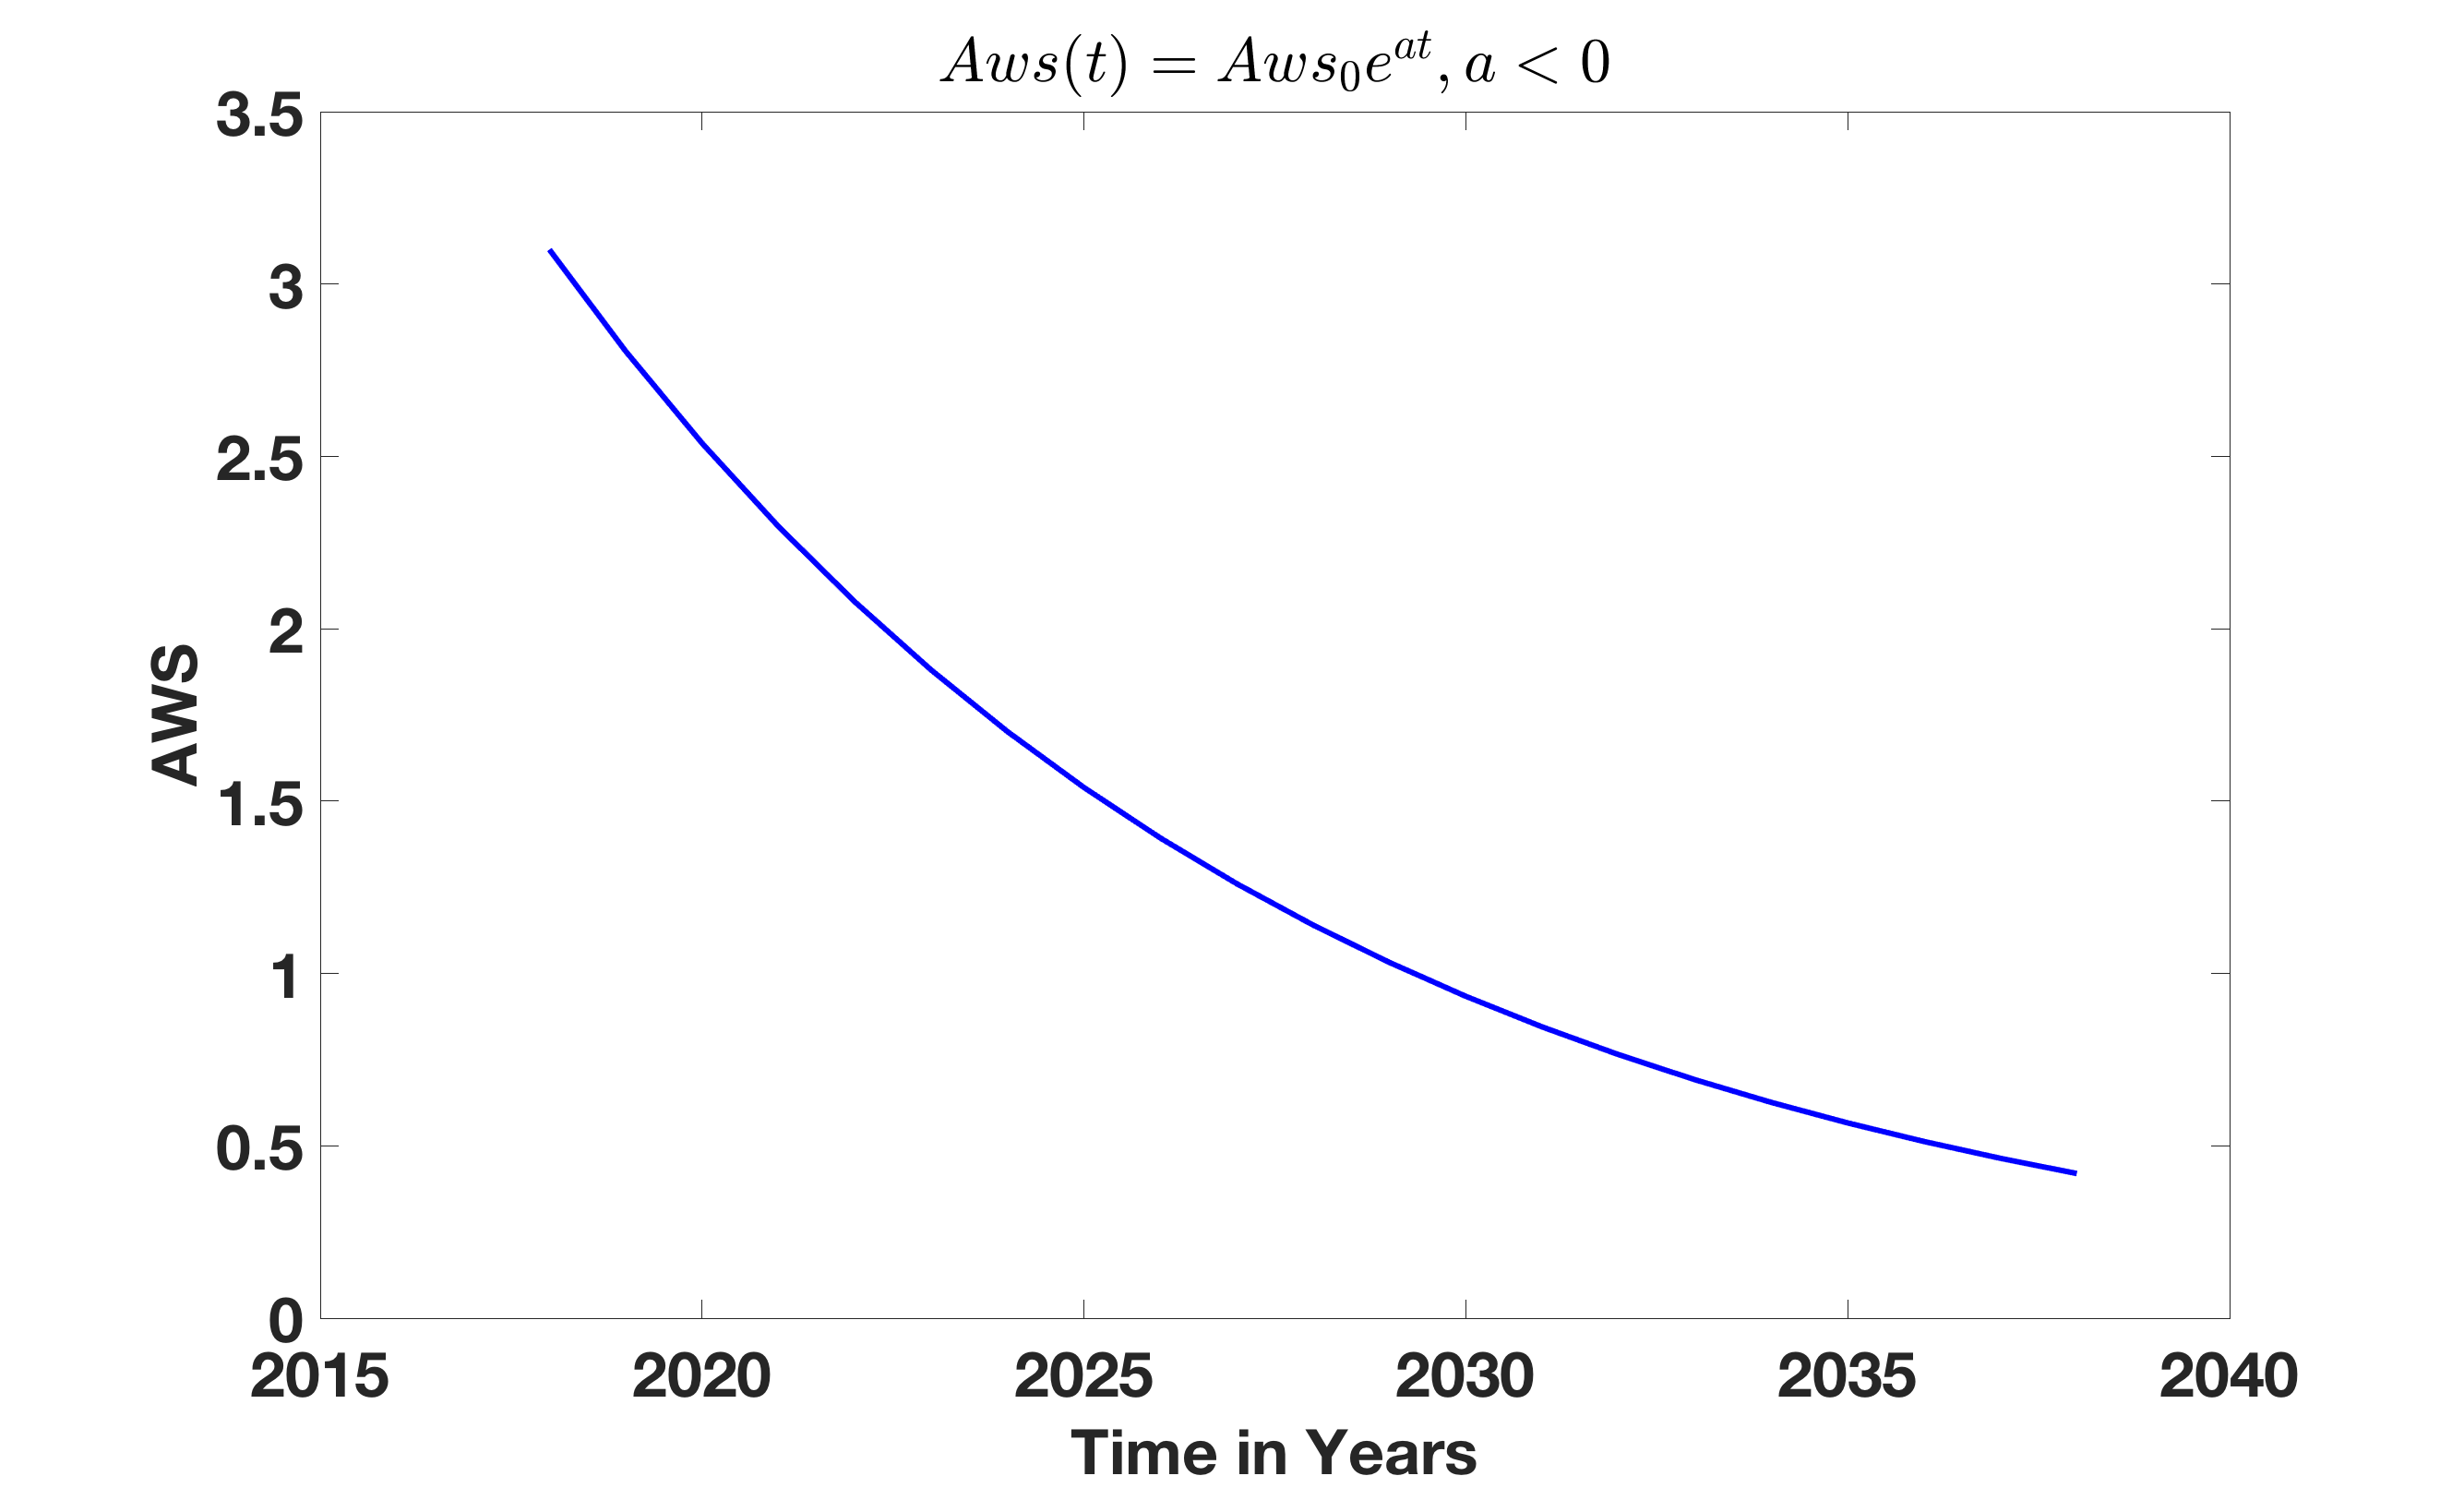
\includegraphics[width=\linewidth]{awsincome1}
\caption{Operating income(in Billons USD)of AWS when $a < 0$}
\label{fig:awsincome1}
\end{figure}

\begin{figure}[ht]\centering
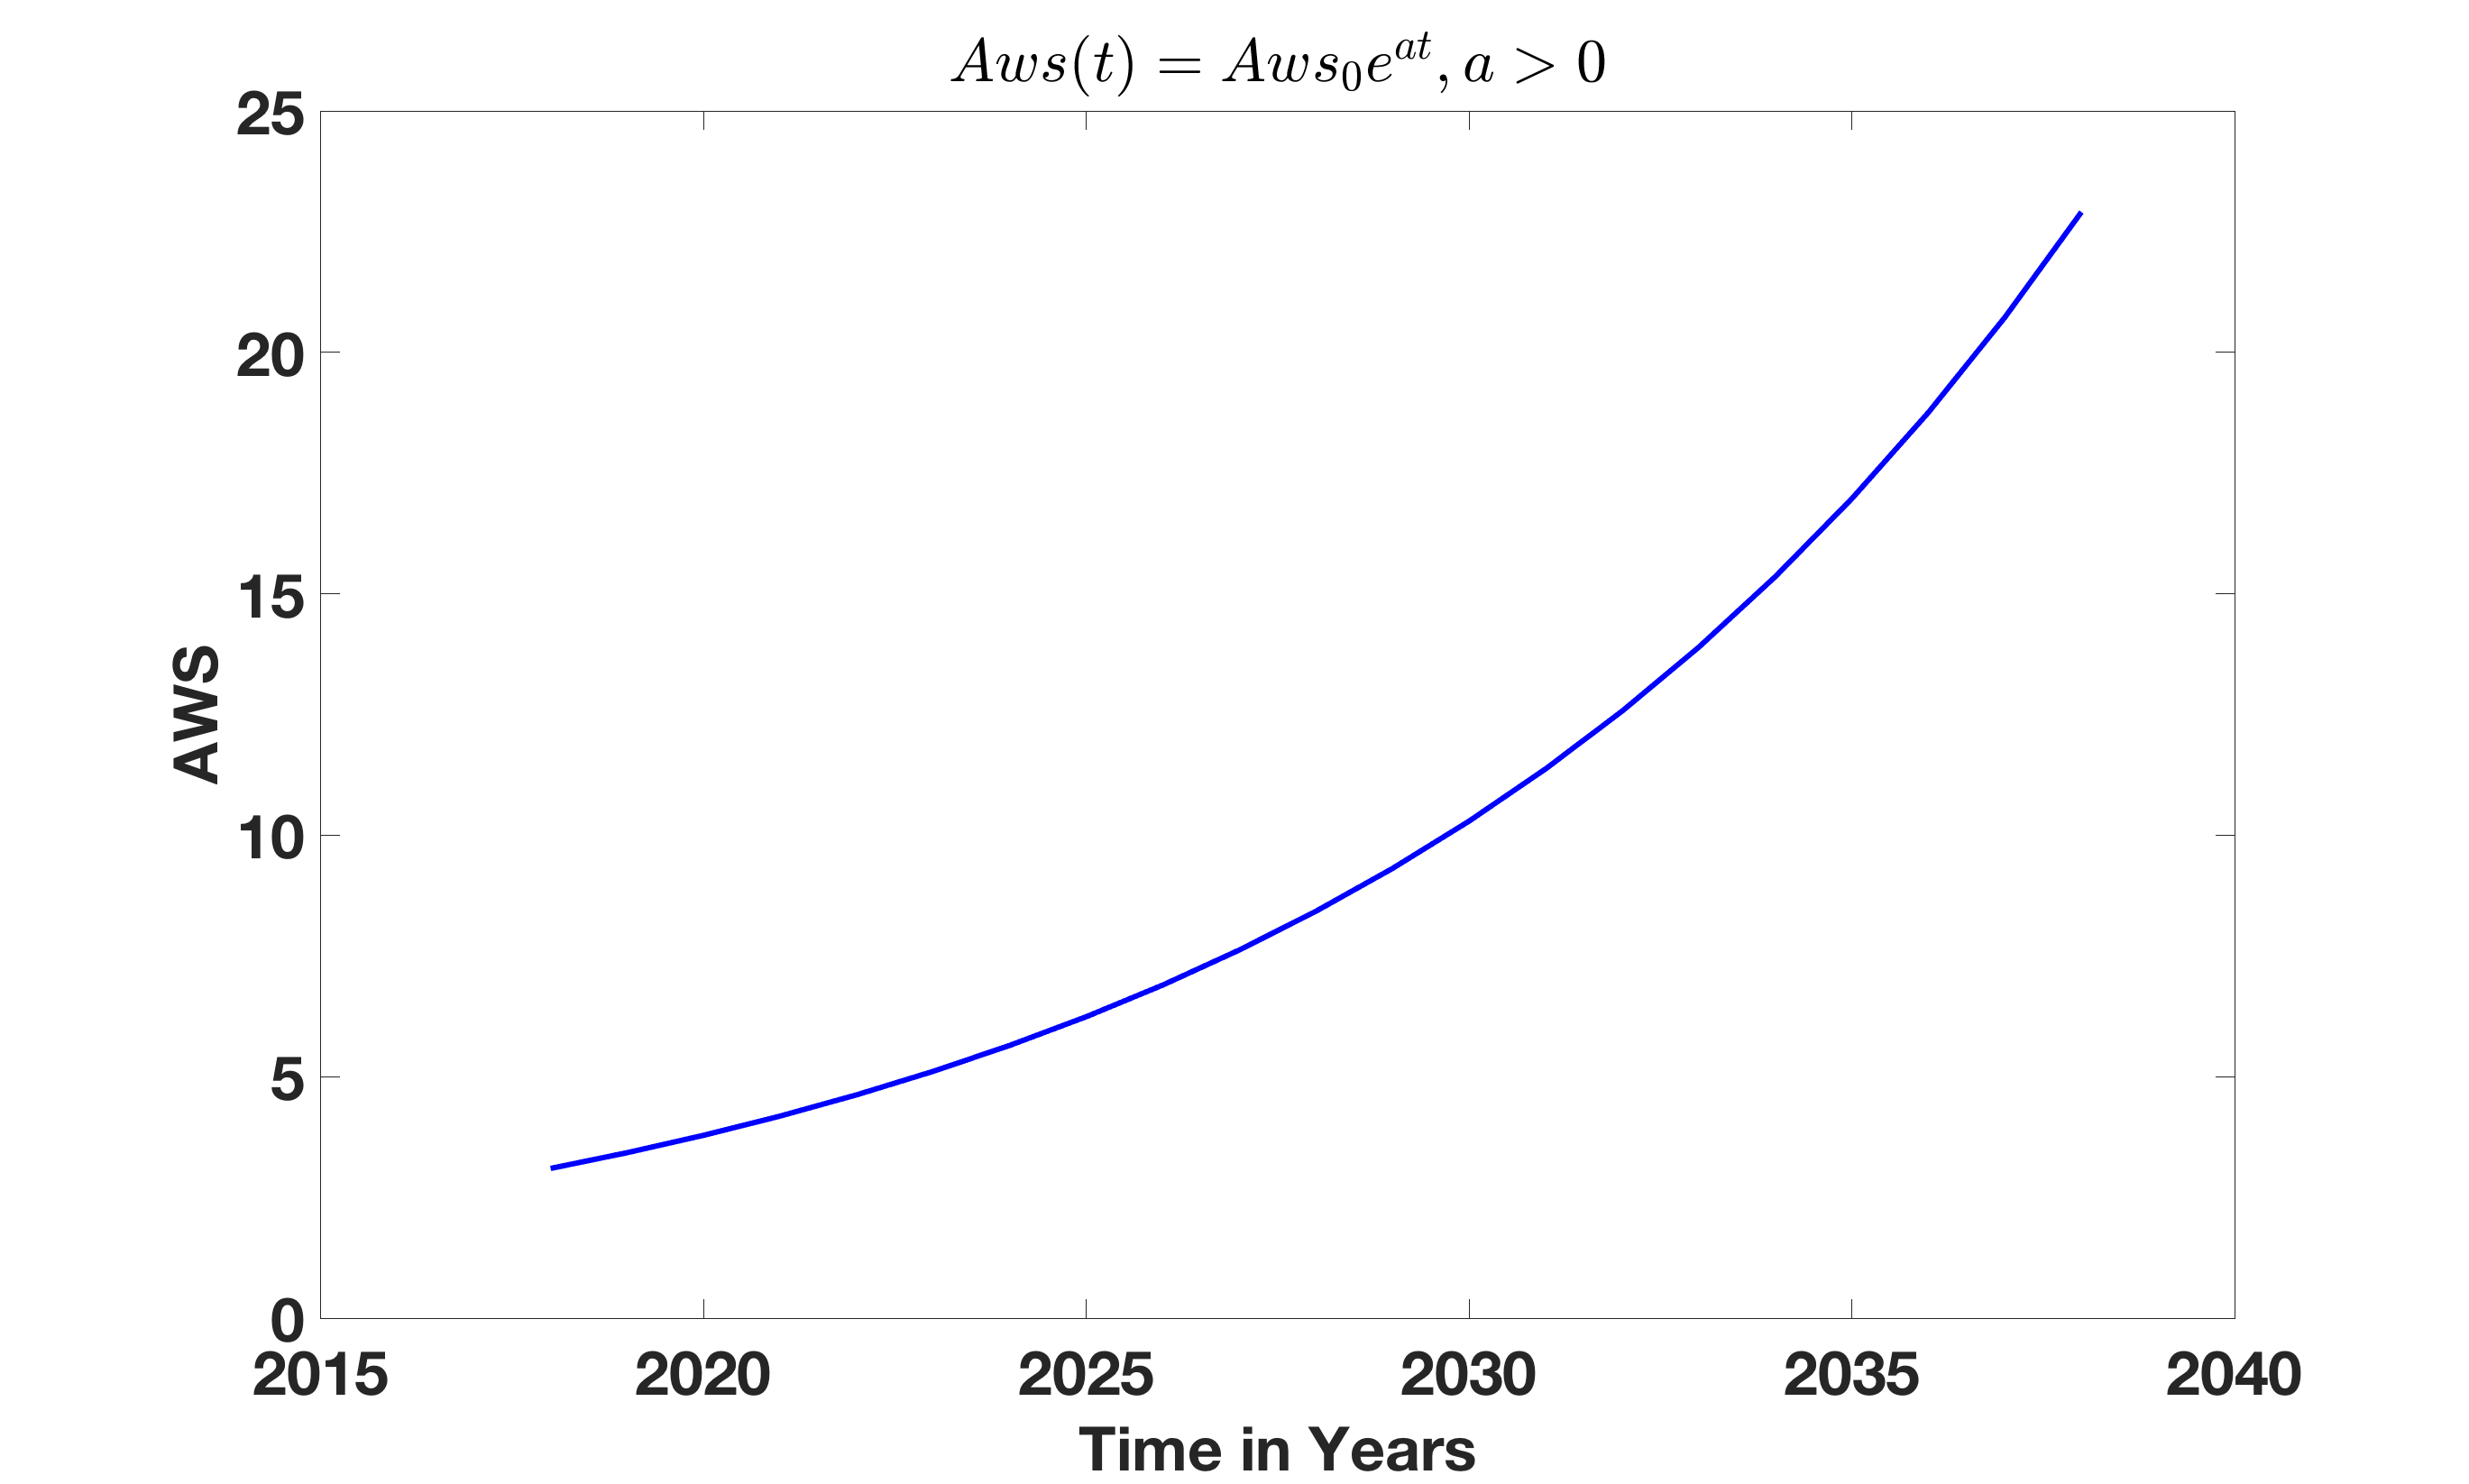
\includegraphics[width=\linewidth]{awsincome2}
\caption{Operating income(in Billons USD)of AWS when $a > 0$}
\label{fig:awsincome2}
\end{figure}

The model is written in a matrix format and given below.
\[
\centering
\begin{bmatrix} 
\dot{Aws} \\
\dot{Amz}
\end{bmatrix}
=
\begin{bmatrix}
a & b \\
c & d
\end{bmatrix}
\begin{bmatrix}
Aws\\
Amz
\end{bmatrix}
\]

\begin{equation} \centering
\dot{X} = AX
\label{eq:mateqe}
\end{equation}
Where,
\[
\dot{X} =
\begin{bmatrix}
\dot{Aws} \\
\dot{Amz}
\end{bmatrix}
,A=
\begin{bmatrix}
a & b \\
c & d
\end{bmatrix}
,X=
\begin{bmatrix}
Aws\\
Amz
\end{bmatrix}
\]
A is a square matrix, $\lambda$ is the eigen value of square matrix A and the characteristic polynomial of a square matrix A is defined as $p(\lambda) = det(A-\lambda I)$. 
\[
\centering
p(\lambda) =
\begin{bmatrix} 
a - \lambda & b \\
c & d - \lambda
\end{bmatrix}
\]
\begin{equation} \centering
\begin{split}
p(\lambda) & = \lambda^2 - (a + d)\lambda + (ad - bc) \\
&= \lambda^2 - (Tr A)\lambda + Det(A) \\
&= \lambda^2 - T\lambda + D
\end{split}
\label{eq:lambda1}
\end{equation}
T is called the trace of matrix A and D is the determinant of the matrix A.

Then looking for the full quadratic formulat for $p(\lambda) = 0$,
\begin{equation} \centering
\lambda  = \frac{-T\pm \sqrt{(T^2 - 4D)}}{2}
\label{eq:lambda2}
\end{equation}
we can determine the conditions or the sign in the case of real eigenvalues and also the signs of real part of the complex case. 

\begin{enumerate}
\item If $D < 0$, the eigenvalues are real and of opposite sign, and the phase portrait is a saddle
\item If $0<D<\frac{T^2}{4}$, the eigenvalues are real, distinct, and of the same sign, and the phase portrait is a node, stable if $T < 0$, unstable if $T>0$
\item If $0 < \frac{T^2}{4} < D$, the eigenvalues are neither real nor purely imaginary, and the phase portrait is a spiral, stable if $T < 0$, unstable if $T > 0$
\end{enumerate}

\begin{figure}[ht]\centering
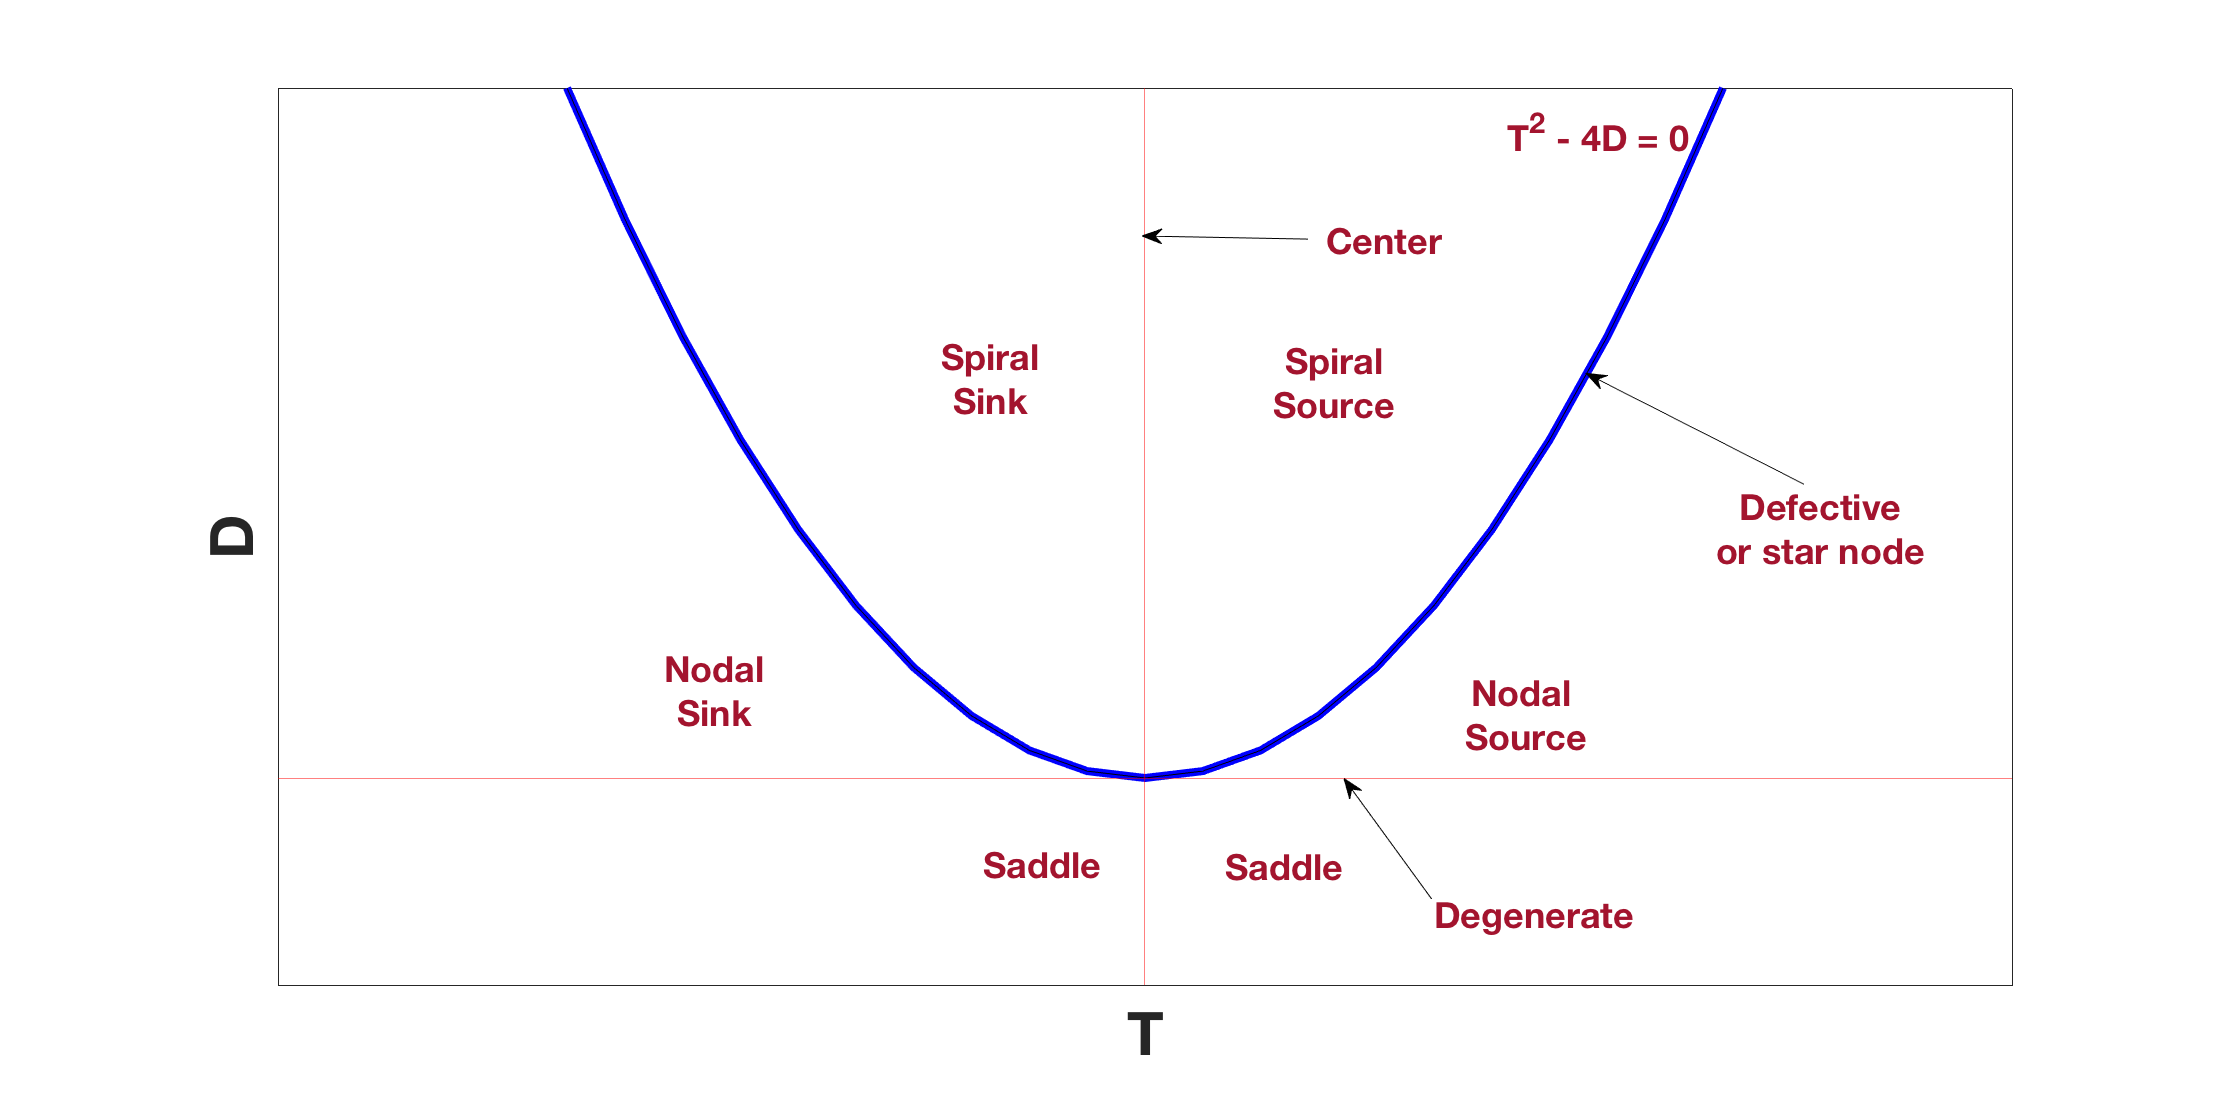
\includegraphics[width=\linewidth]{gpport}
\caption{Phase Plane}
\label{fig:gpport}
\end{figure}

For all roots of real and distinct, each eigen value $\lambda_i$ has one associated eigenvector $V_i$. These vectors form a set of linearly independent solutions. 

\begin{equation} \centering
\begin{split}
X_1(t) &= e^{\lambda_1 t}V_1  \\
X_2(t) &= e^{\lambda_2 t}V_2
\end{split}
\label{eq:ge}
\end{equation}

The general solution is given by 

\begin{equation} \centering
X(t) = C_1 e^{\lambda_1 t}V_1 + C_2 e^{\lambda_2 t}V_2
\label{eq:ge2}
\end{equation}

Where $C_1,C_2$ are arbitrary constants and can be determined based on the initial conditions $X(0)$. When $t=0$,
\begin{equation} \centering
X(0) = C_1 V_1 + C_2 V_2  
\label{eq:ge3}
\end{equation}
\[
\begin{bmatrix}
X_1(0) \\ 
X_2(0) 
\end{bmatrix}
=
\begin{bmatrix}
V_1 & V_2
\end{bmatrix}
\begin{bmatrix}
C_1 \\
C_2
\end{bmatrix}
\]

$X_1(0)$ and $X_2(0)$ are the operating income of AWS and Amazon North America as given in the table \ref{table:income},value of $C_1$ and $C_2$ can be obtained by solving two linear equations.  

\[
\begin{bmatrix}
3.10 \\
2.36  
\end{bmatrix}
=
\begin{bmatrix}
V_1 & V_2
\end{bmatrix}
\begin{bmatrix}
C_1 \\
C_2
\end{bmatrix}
\]
A general framework has been established to understand the long term dynamics of AWS and Amazon North America. By selecting possible scenario by selecting the appropriate values for $a,b,c,d$ which leads into the value of $D$ and $T$, the framework can be used to understand the long term dynamics of both AWS and Amazon North America organization. 

%------------------------------------------------

\section{Results and Discussion}

\subsection{Scenarios}

\textbf{Scenario \#1 - Run alone at steady speed:}
In this scenario, the AWS and Amazon North America business units are independent to each other and does not have any positive or negative impact to each other.AWS customer does not have change their cloud provider AWS even when Amazon North America penetrates into their core business. Likewise, the Amazon North America business is not impacted due to AWS growth. For instance, the AWS competitors like Google or Microsoft employees continue to use Amazon North America services even when they compete with AWS business unit.
\[
A =
\begin{bmatrix}
0.1 & 0.0 \\
0.0 & 0.1
\end{bmatrix}
\]
\begin{figure}[ht]\centering
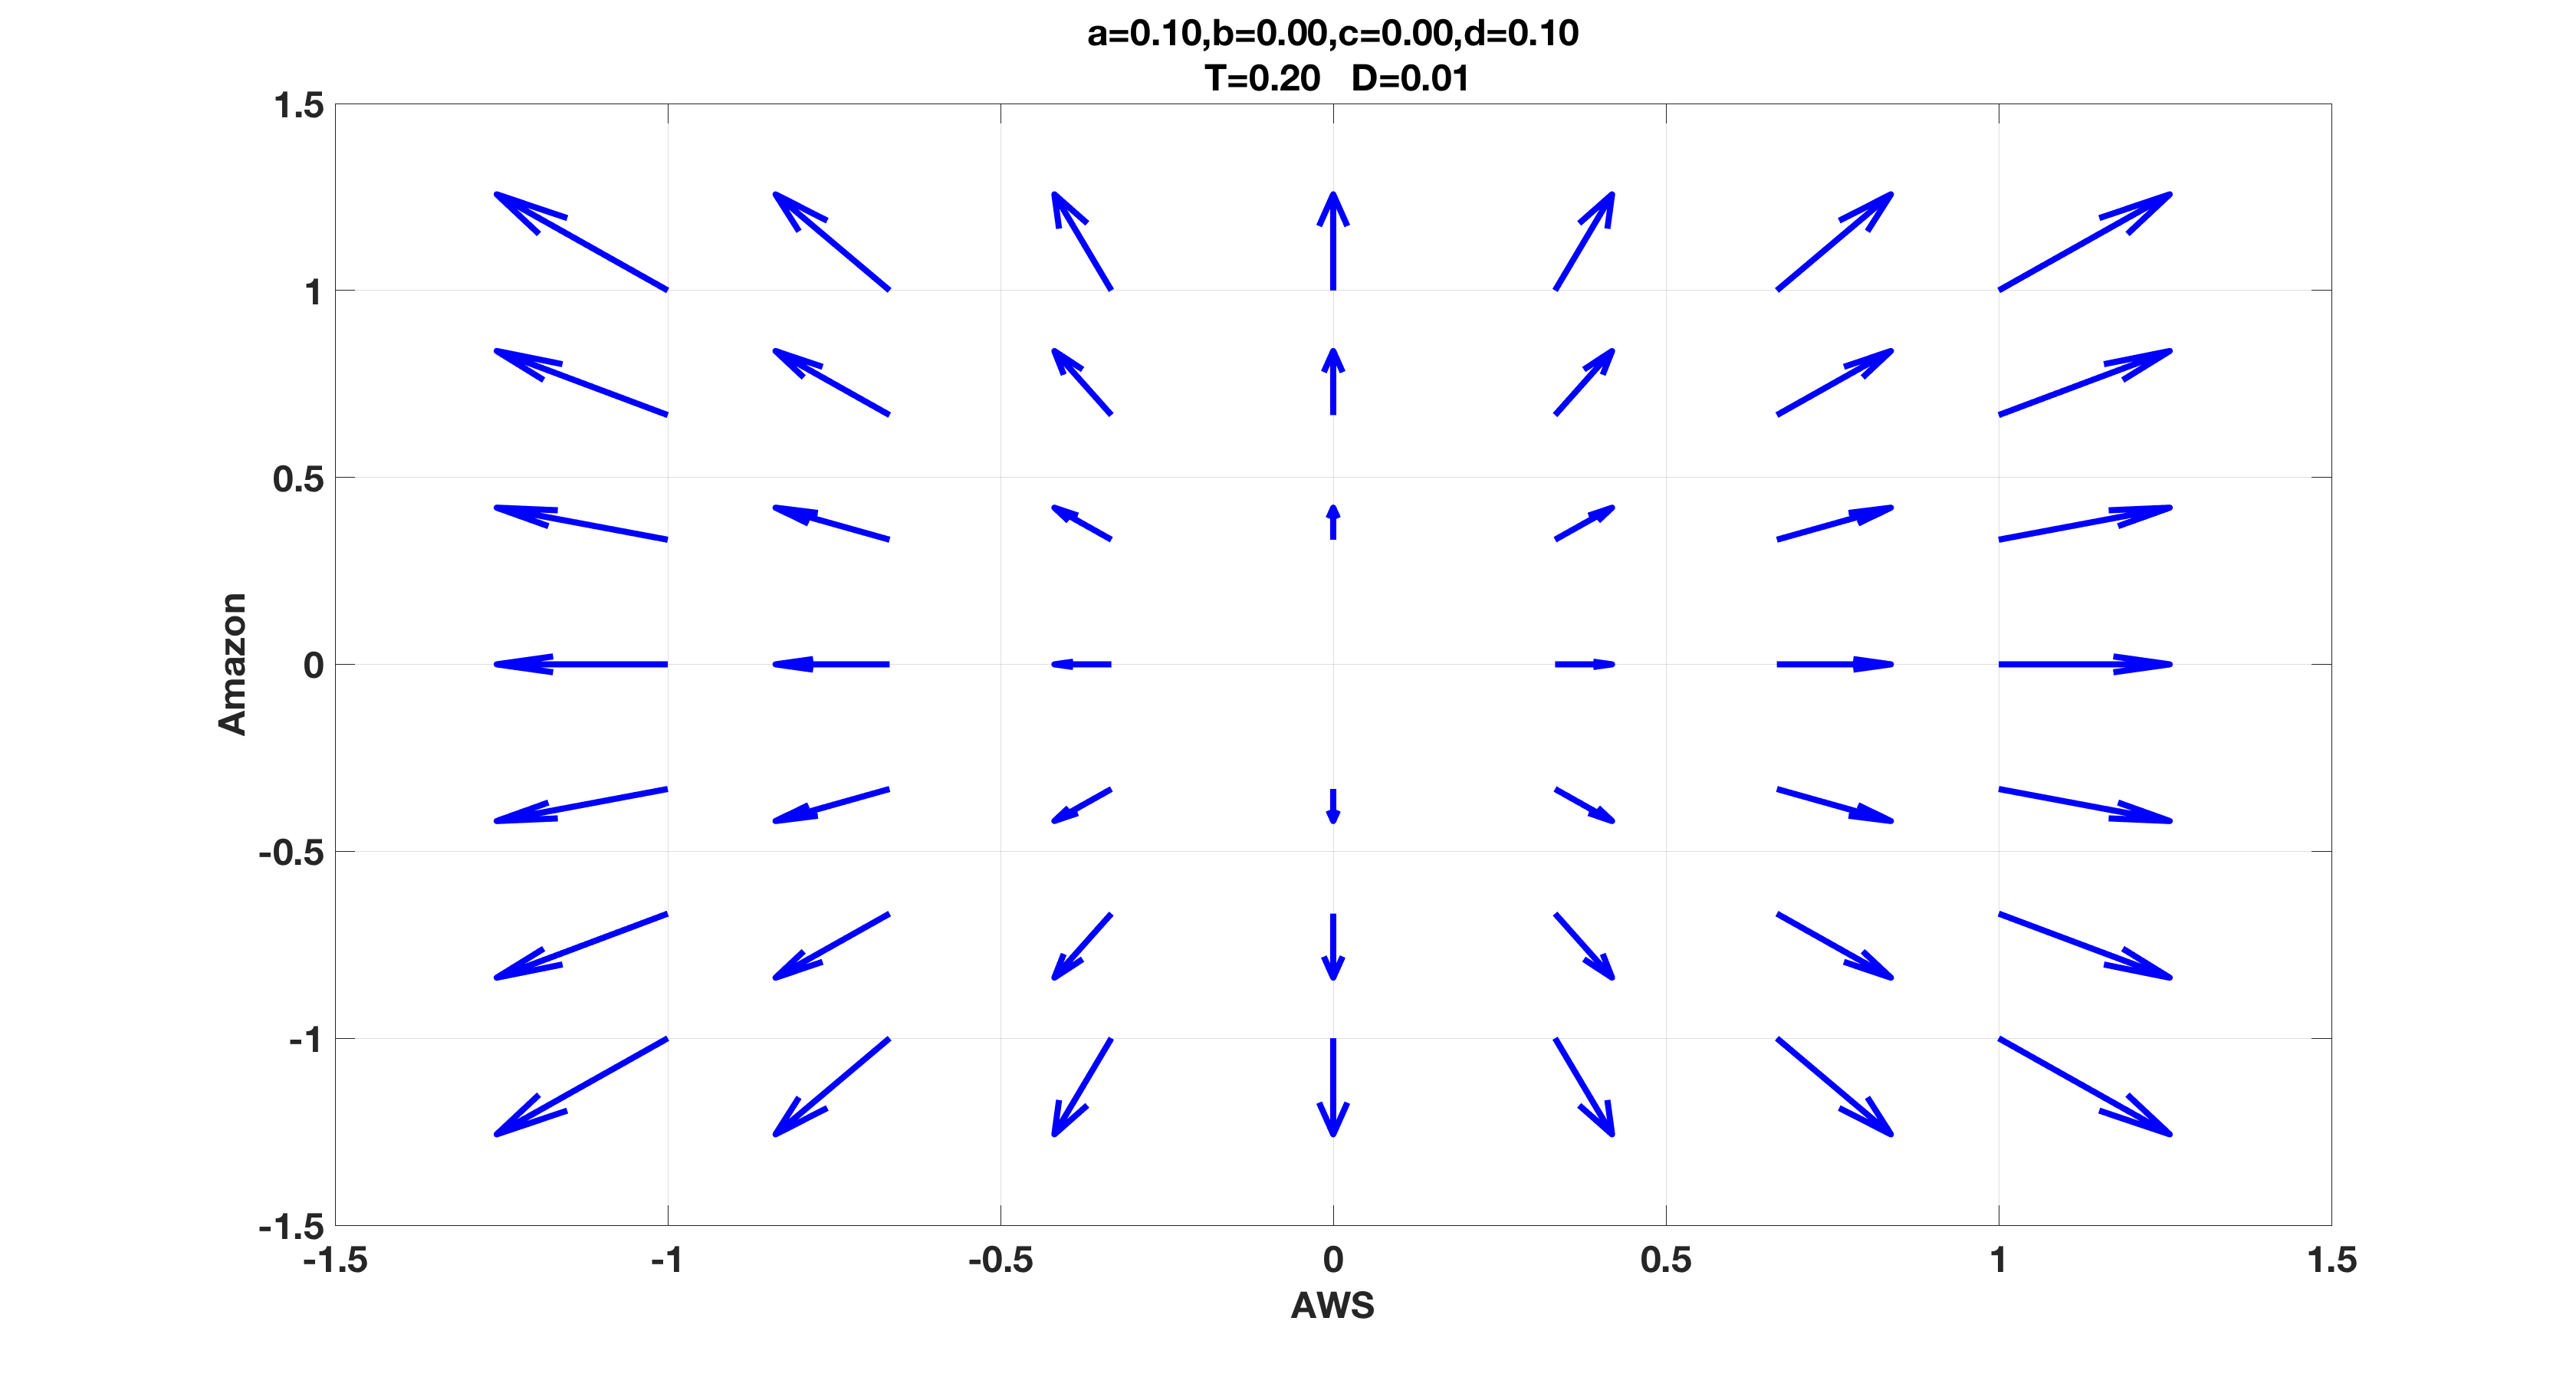
\includegraphics[width=\linewidth]{scen1}
\caption{Phase Portrait for Scenario \#1}
\label{fig:scen1}
\end{figure}  
Eigen values are $\lambda_1 = 0.1$ and $\lambda_2 = 0.1$ and Eigen vectors are given 
\[
V_1 =
\begin{bmatrix}
1  \\
0 
\end{bmatrix}
,V_2 =
\begin{bmatrix}
0  \\
1 
\end{bmatrix}
\]
In this case $C_1$ and $C_2$ is same as the $X_1(0)$ and $X_2(0)$ respectively. 

The phase portrait is given in the figure \ref{fig:scen1} and implies that both the units exponentially grow in long term. 

\textbf{Long term Operating Income for Scenario \#1}
By using the framework established and the conditions set for this scenario based on $a$,$b$,$c$,$d$, the general operating income equation for Amazon (including the North America and AWS) are given below. 
\begin{equation} \centering
X(t) = 3.1 e^{0.1 t} + 2.36 e^{0.1 t}
\label{eq:s1}
\end{equation}

\begin{figure}[ht]\centering
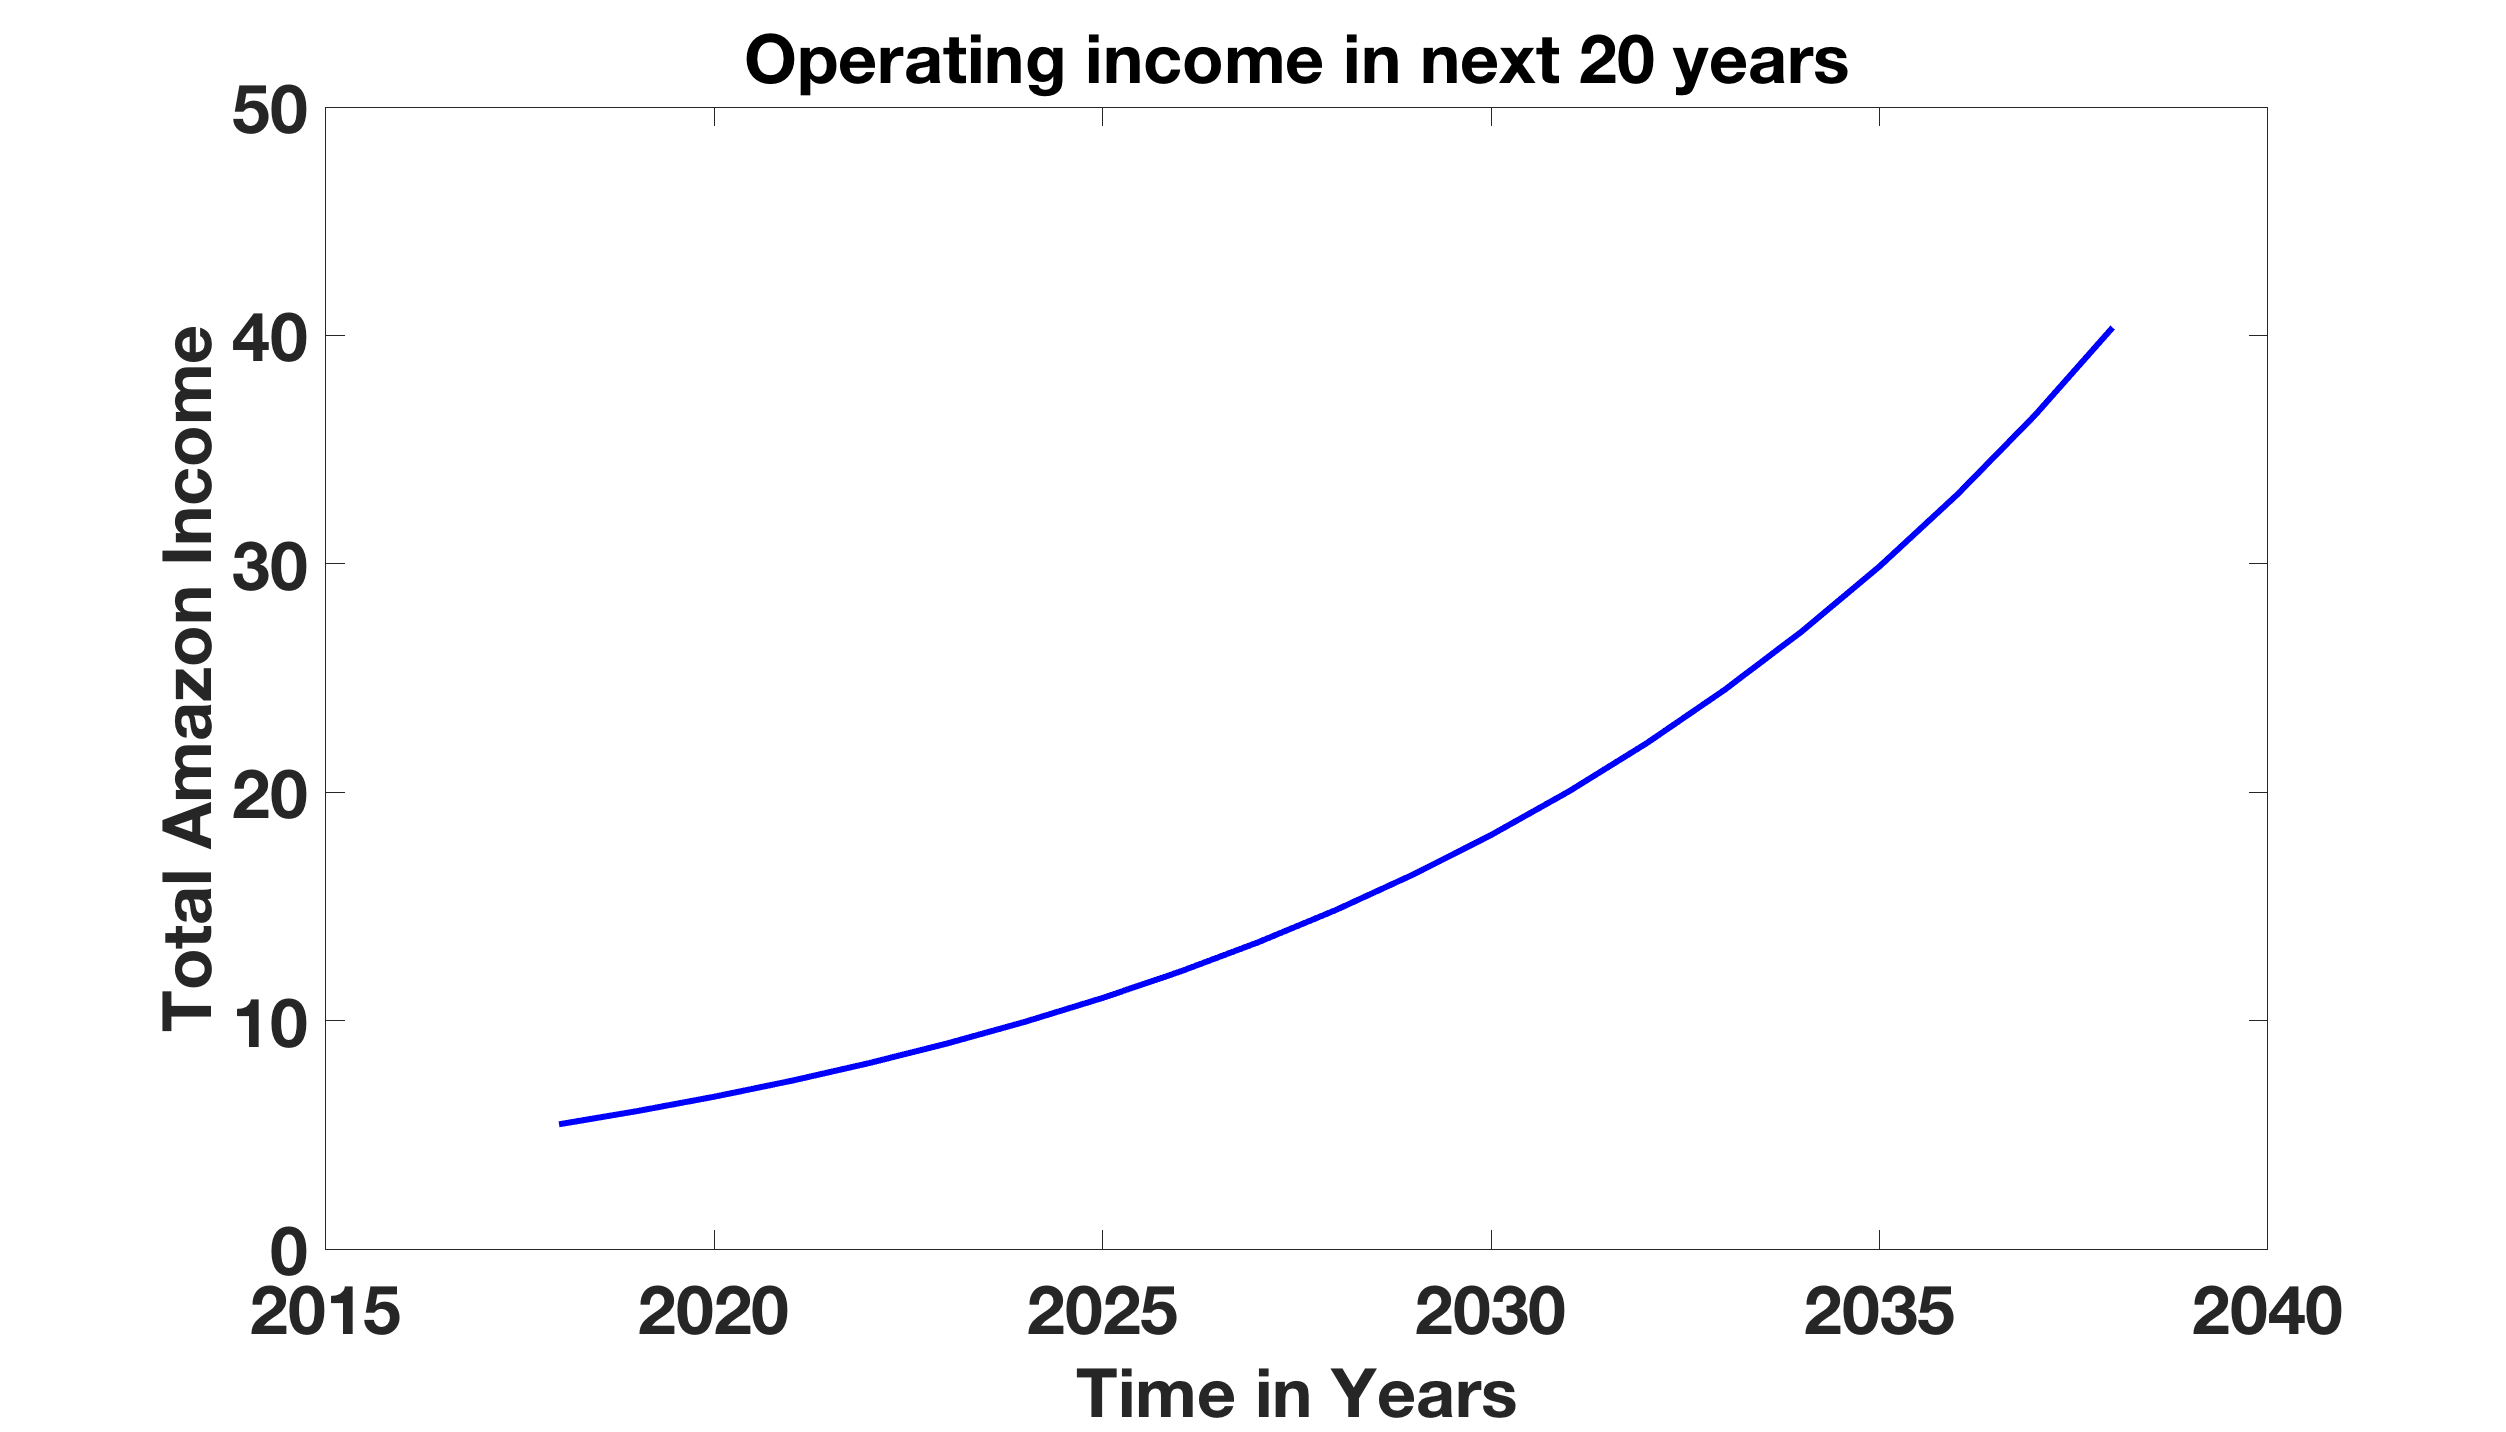
\includegraphics[width=\linewidth]{scen1income}
\caption{Operating income (USD, Billions) for next 20 years for Scenario \#1}
\label{fig:scen1income}
\end{figure}

The figure \ref{fig:scen1income} represents the operating income of Amazon for next 20 years. 

\textbf{Scenario \#2 - Fear of competition:}
In this scenario, the AWS customer has a fear that Amazon North America penetrates into their core business, disrupt their business model and make them irrelevant in the market place in long run. This scenario happened for companies like Borders, ToyRus and the scenario is real. Due to the potential competitive threat from Amazon, a percentage of AWS's customer pull out of AWS customer service and seek out an alternative cloud provider like Microsoft or Google.Likewise, the Amazon North America business is impacted due to AWS growth. For instance, few percentage of the AWS competitors like Google or Microsoft employees discontinue to use Amazon North America services and the employees who feels Amazon's threat in their core business limits their use of Amazon North America. 
\[
A =
\begin{bmatrix}
0.1 & -0.05 \\
-0.01 & 0.1
\end{bmatrix}
\]
\begin{figure}[ht]\centering
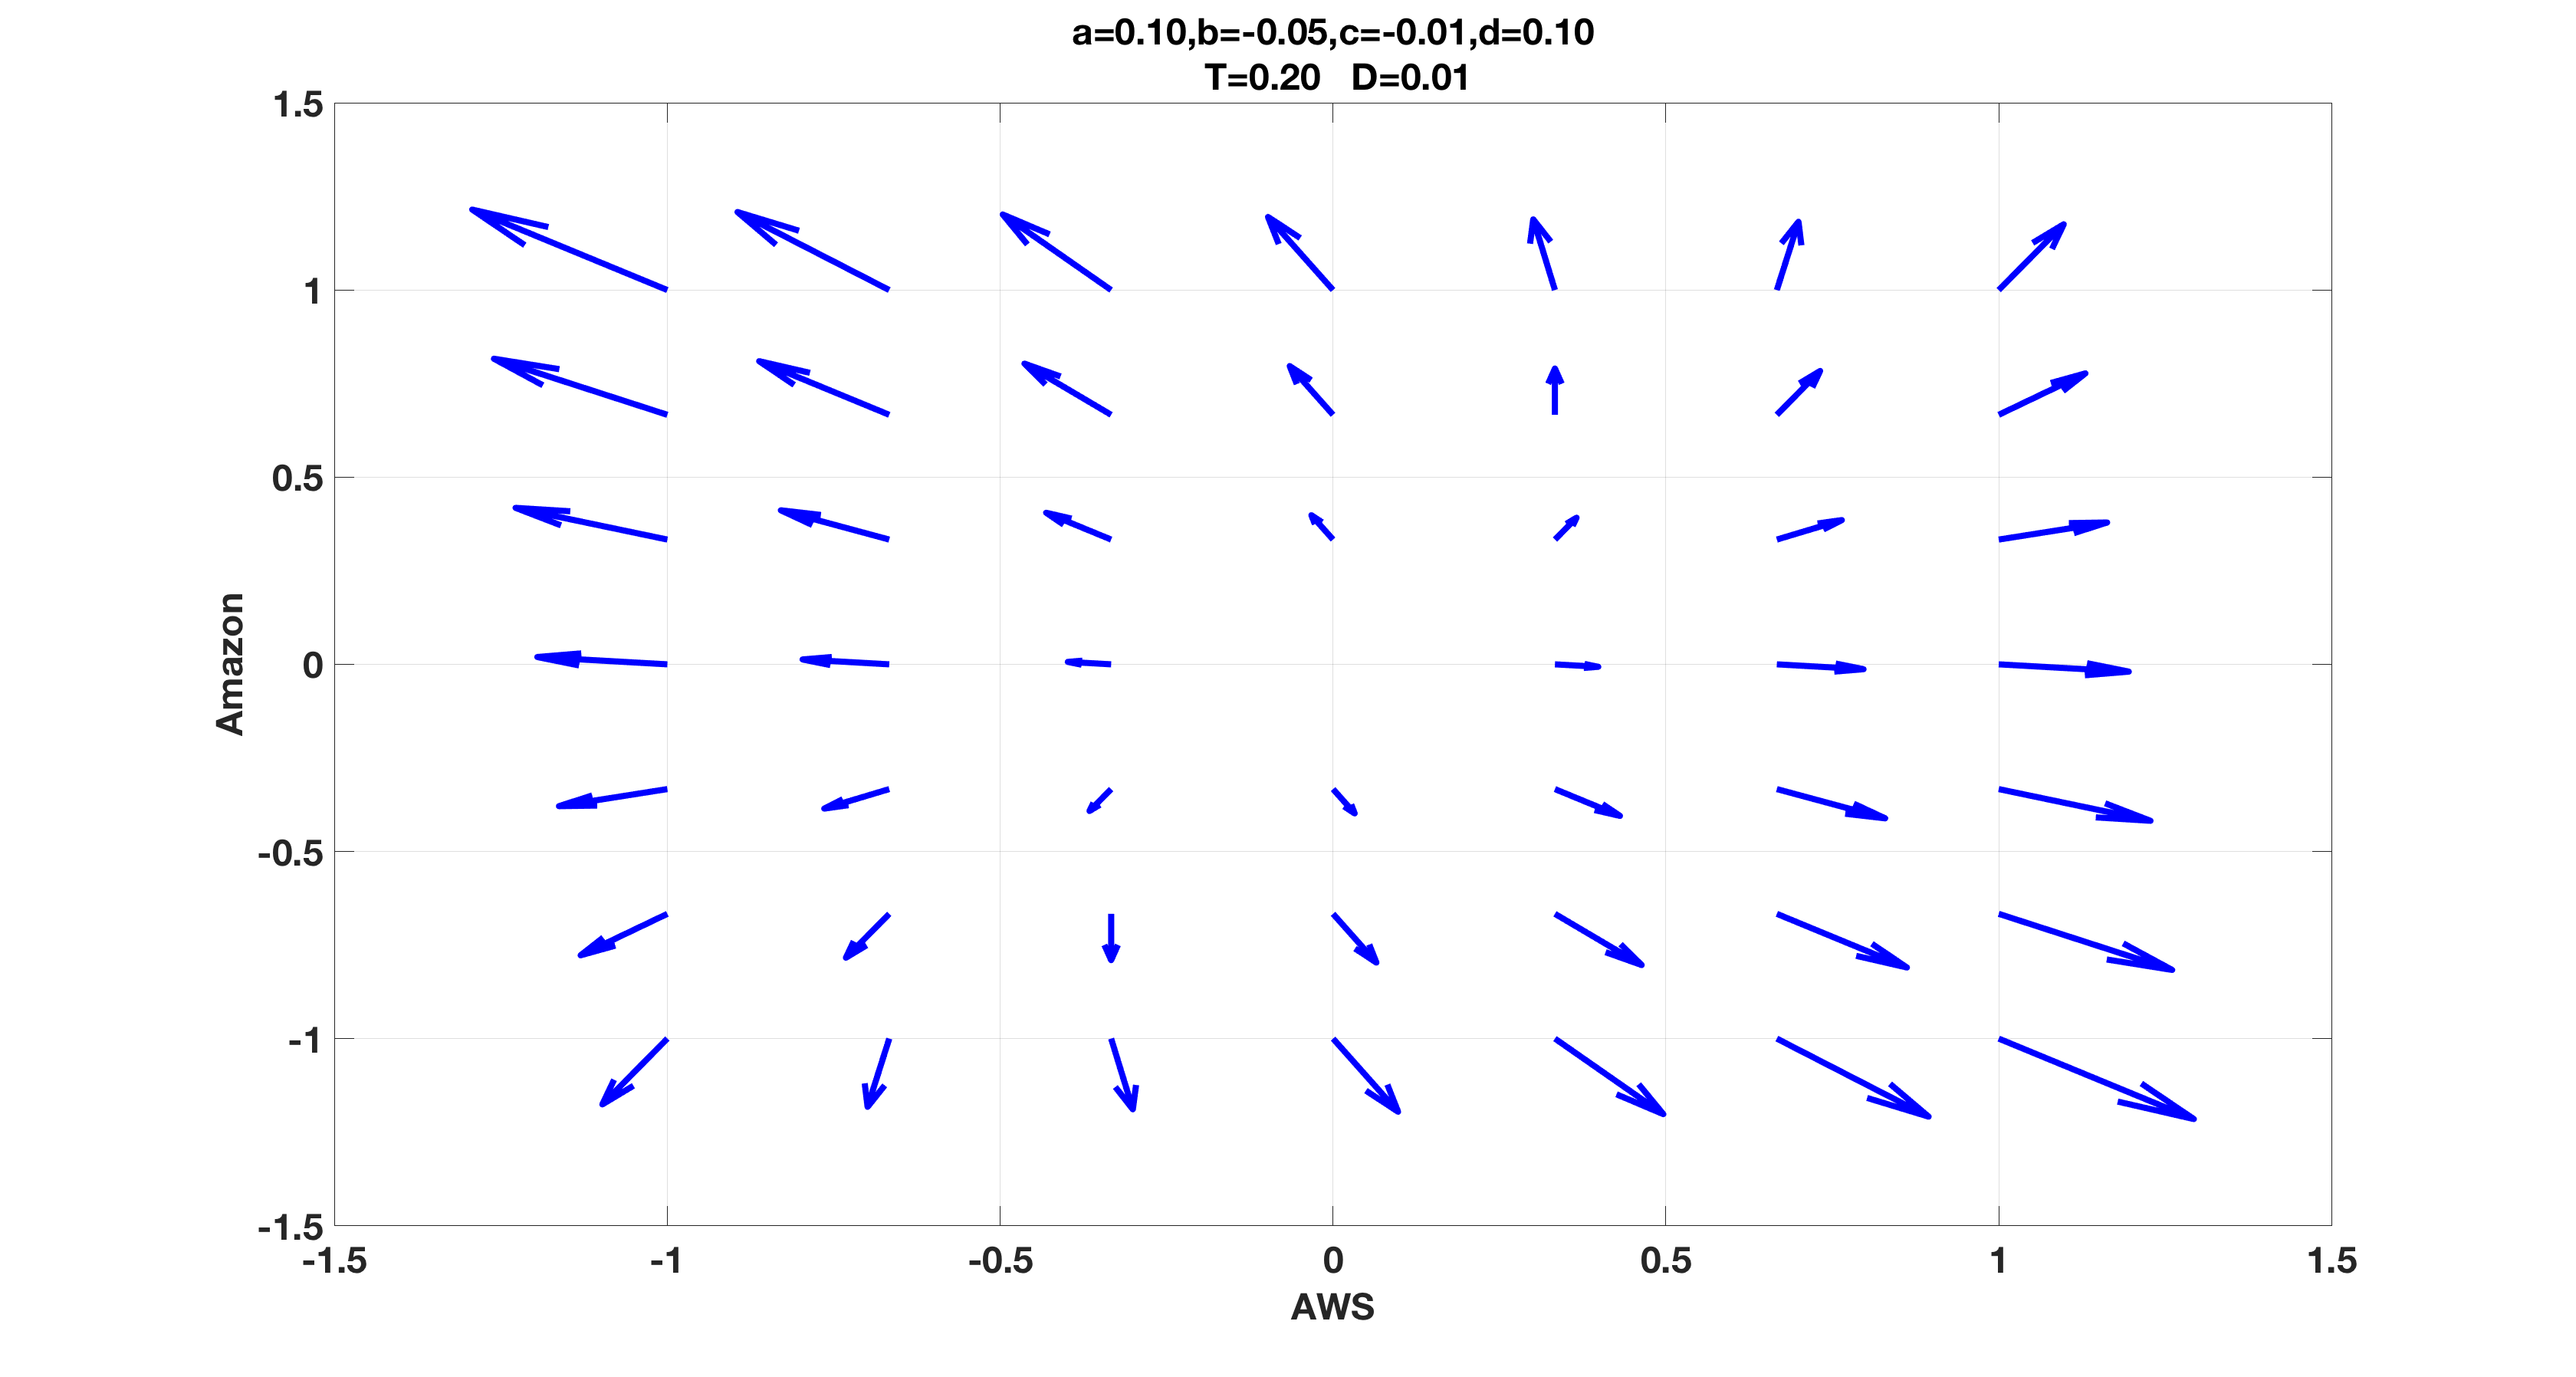
\includegraphics[width=\linewidth]{scen2}
\caption{Phase Portrait for Scenario \#2}
\label{fig:scen2}
\end{figure}  
Eigen values are $\lambda_1 = 0.1447$ and $\lambda_2 = 0.0553$ and Eigen vectors are given 
\[
V_1 =
\begin{bmatrix}
0.7454  \\
-0.6667 
\end{bmatrix}
,V_2 =
\begin{bmatrix}
0.7454  \\
0.6667
\end{bmatrix}
\]
By using the initial condition,the values of constants are given as,$C_1=0.3095$ and $C_2=3.8495$.

The phase portrait for this scenario is given in the figure \ref{fig:scen2}.

\textbf{Long term Operating Income for Scenario \#2}
By using the framework established and the conditions set for this scenario based on $a$,$b$,$c$,$d$, the general operating income equation for Amazon (including the North America and AWS) are given below. 
\begin{equation} \centering
X(t) = 0.30^{0.14 t} + 3.84 e^{0.05 t}
\label{eq:s2}
\end{equation}

\begin{figure}[ht]\centering
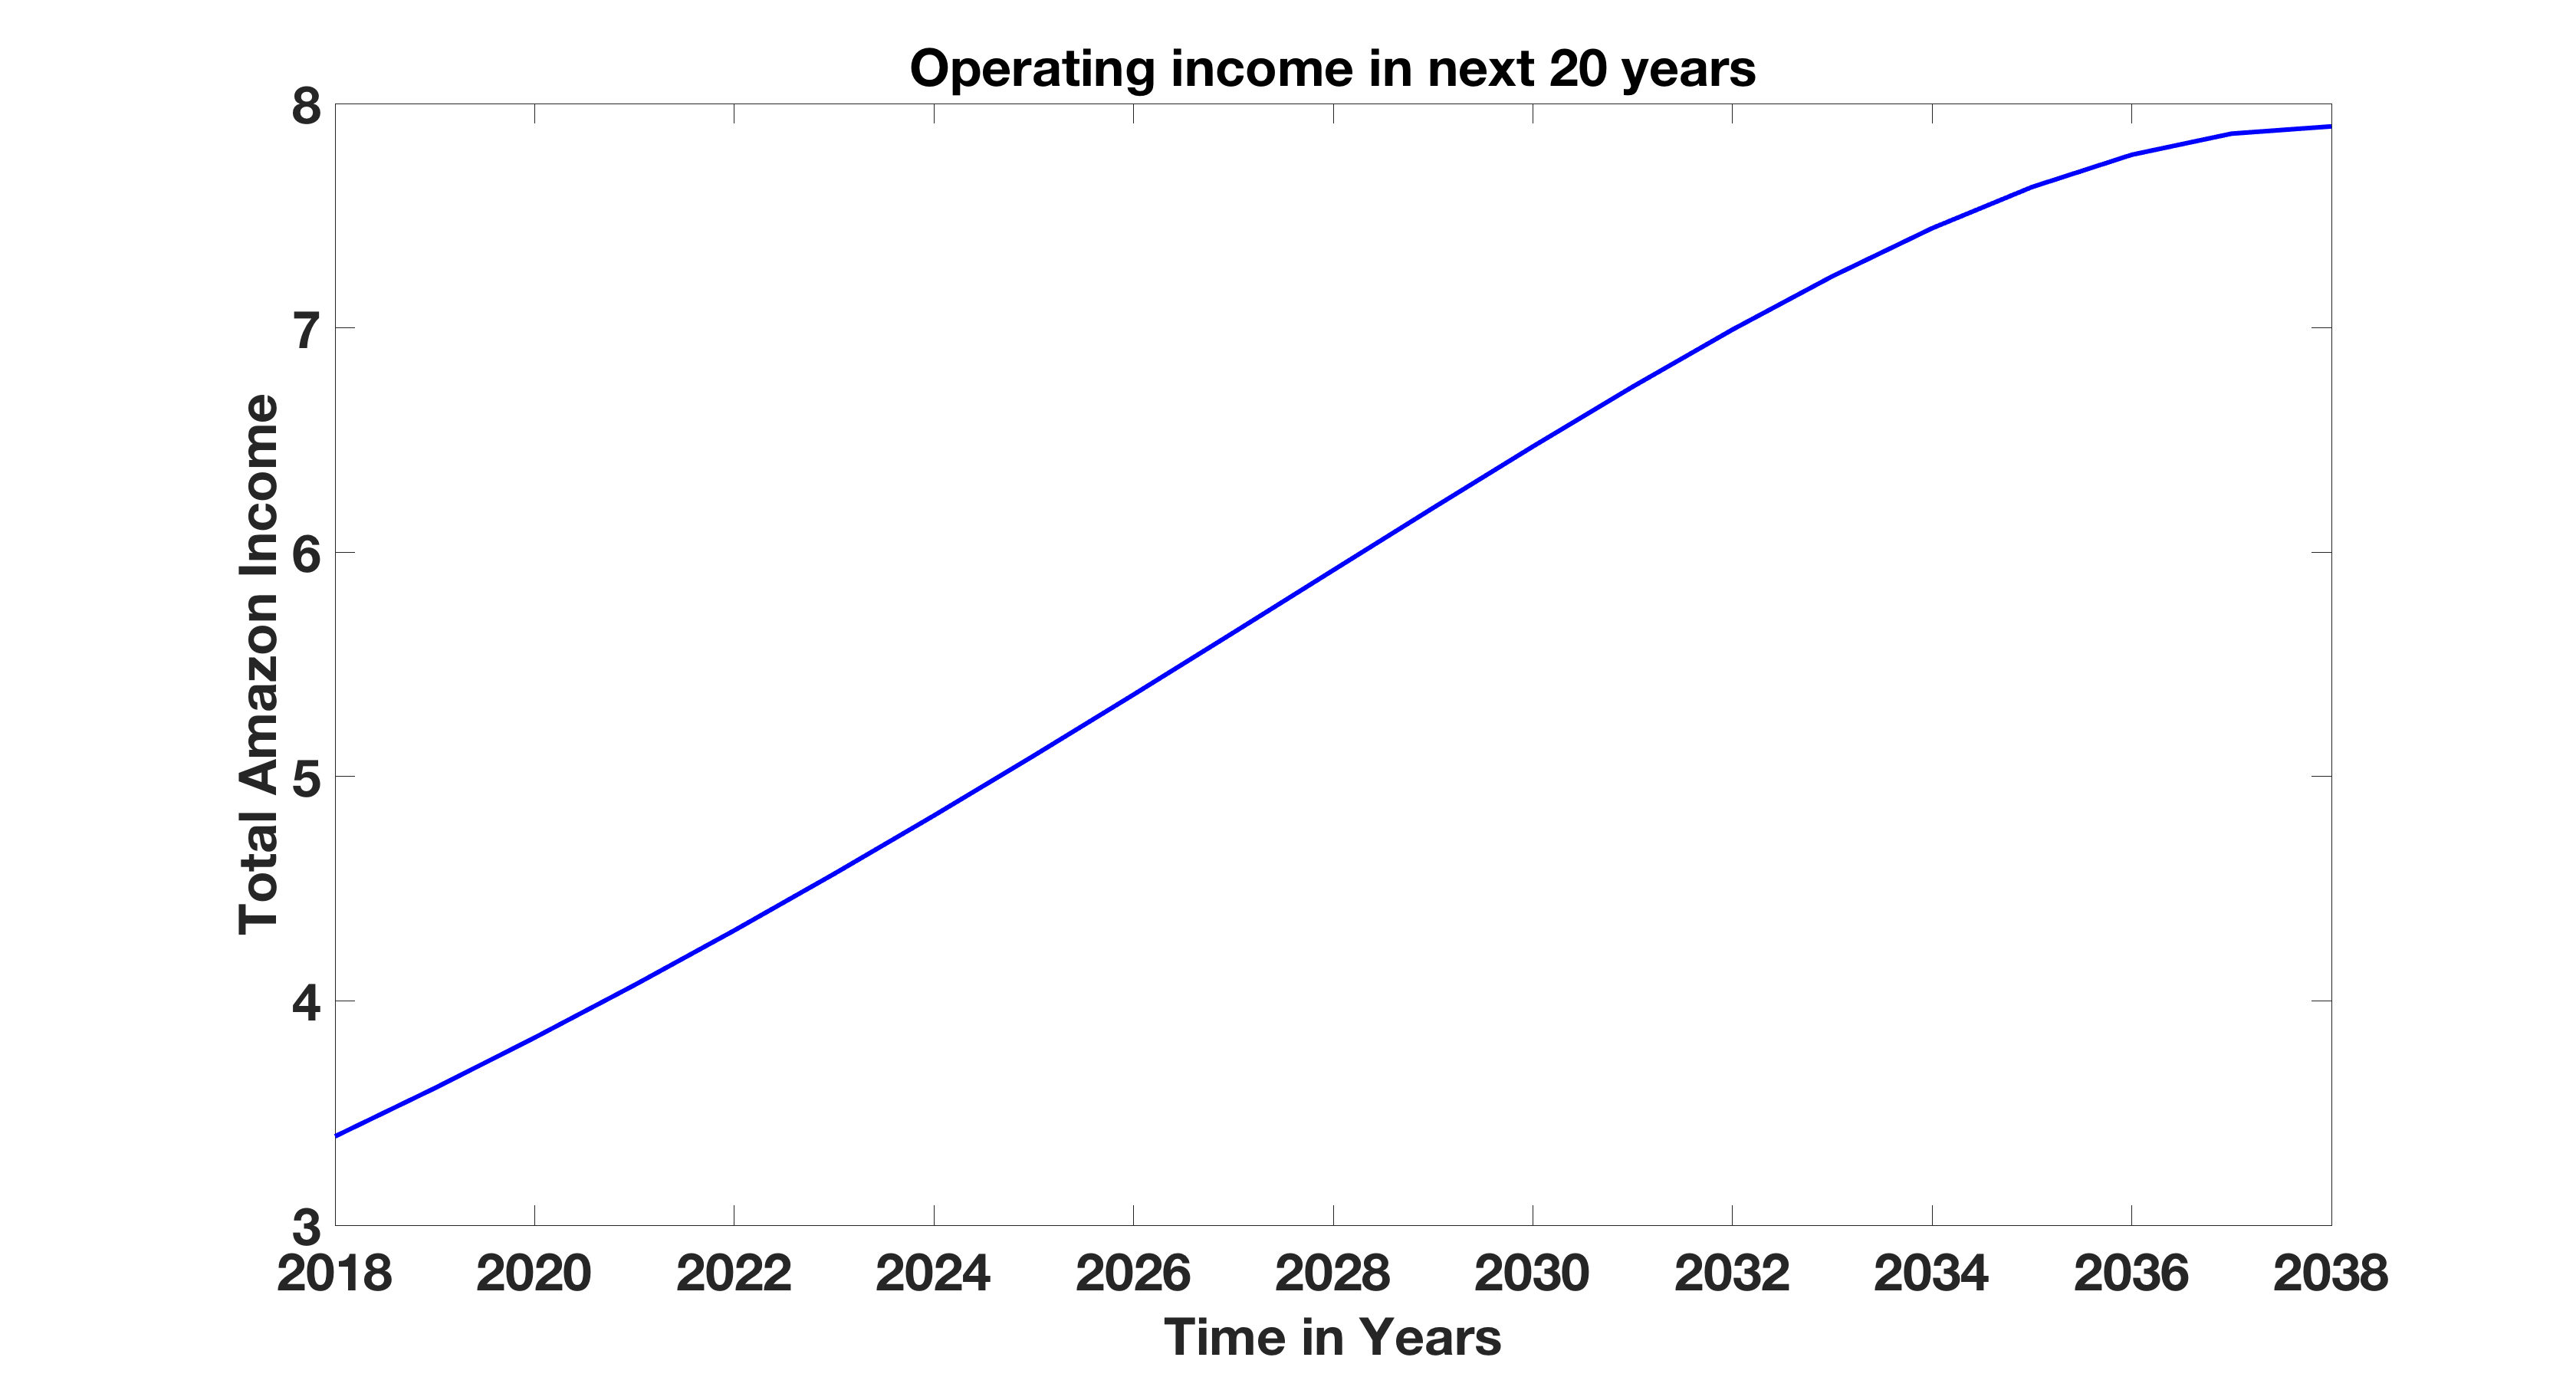
\includegraphics[width=\linewidth]{scen2income}
\caption{Operating income (USD, Billions) for next 20 years for Scenario \#2}
\label{fig:scen2income}
\end{figure}

The figure \ref{fig:scen2income} represents the operating income of Amazon for next 20 years. 


\begin{figure}[ht]\centering
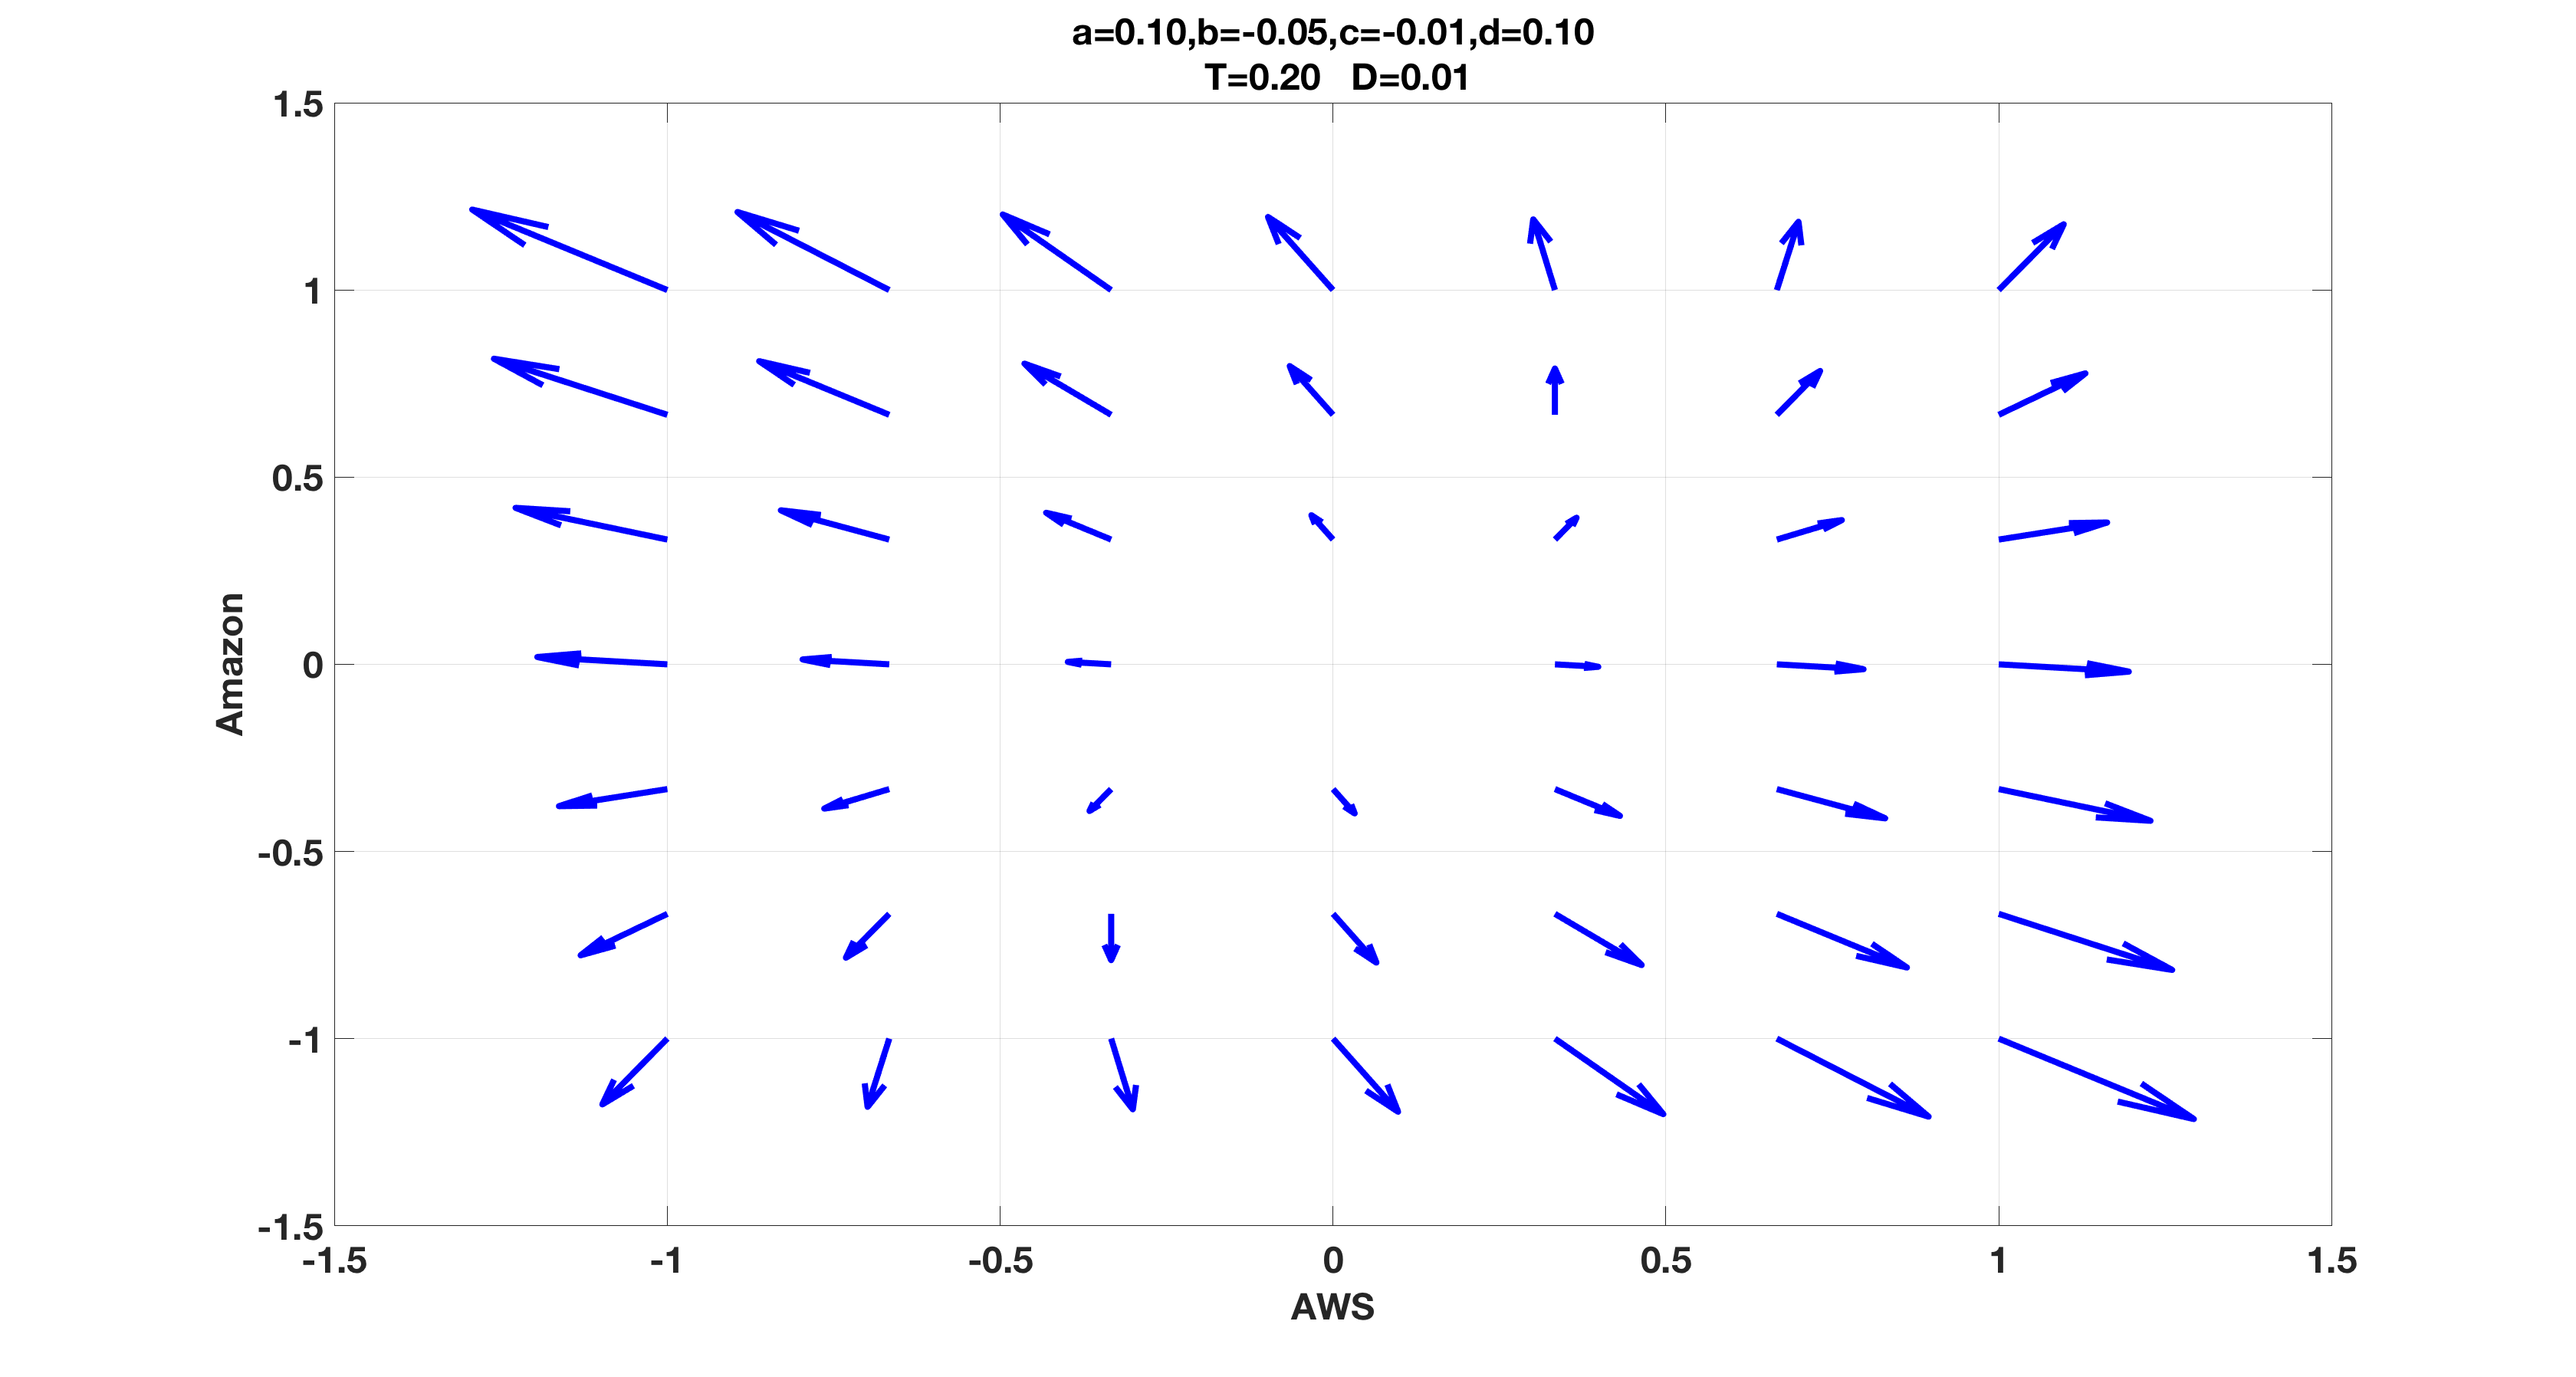
\includegraphics[width=\linewidth]{scen2}
\caption{Phase Portrait for Scenario \#2}
\label{fig:scen2}
\end{figure}
The phase portrait is given in the \ref{fig:scene2} and implies that customer pulling out of AWS due to Amazon North America's penetration into their core business does not have any impact.

\textbf{Scenario \#3 - Excitement of collaboration:}
In this scenario, the AWS customer excited by AWS service and use Amazon North America service more and Amazon North America customers get excited about their market place experience and leverages AWS for their corporate use. In this scenario, the AWS and Amazon's North America's customer provide expand their current usage and start using other service. 
\[
A =
\begin{bmatrix}
0.1 & 0.05 \\
0.01 & 0.1
\end{bmatrix}
\]
\begin{figure}[ht]\centering
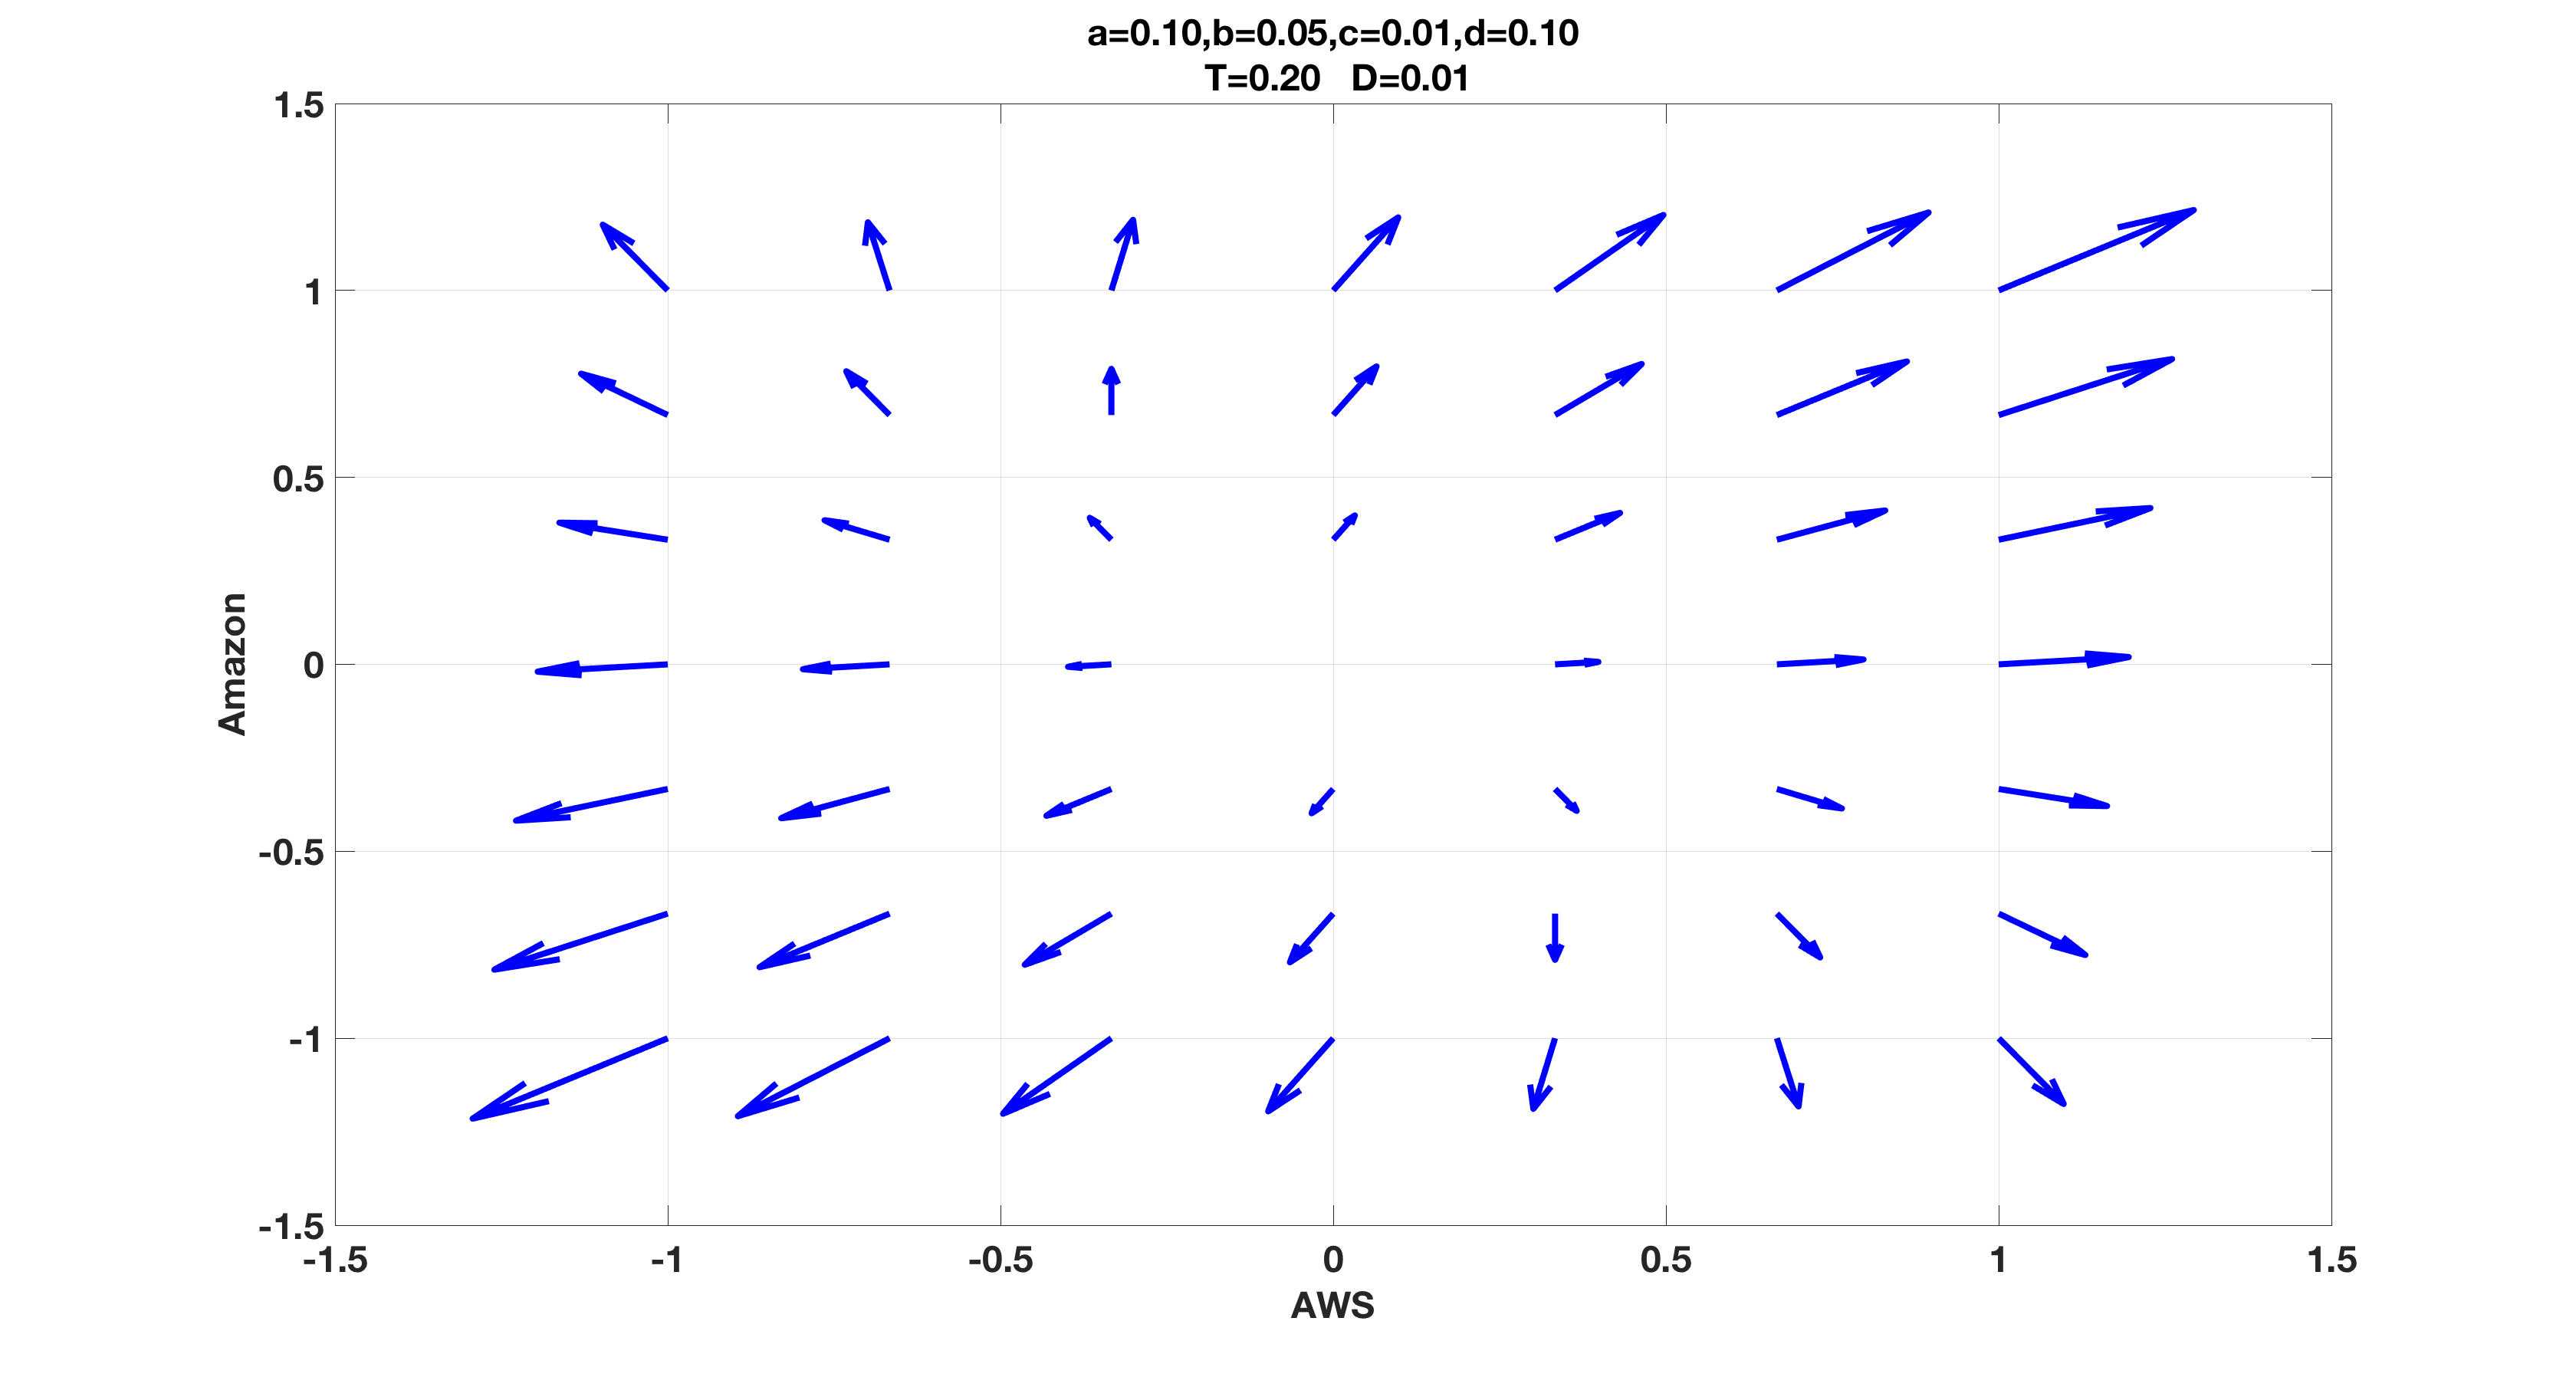
\includegraphics[width=\linewidth]{scen3}
\caption{Phase Portrait for Scenario \#3}
\label{fig:scen3}
\end{figure}  
Eigen values are $\lambda_1 = 0.1224$ and $\lambda_2 = 0.0776$ and Eigen vectors are given 
\[
V_1 =
\begin{bmatrix}
0.9129  \\
0.4082 
\end{bmatrix}
,V_2 =
\begin{bmatrix}
-0.9129  \\
0.4082
\end{bmatrix}
\]
By solving the above equations,$C_1=4.5883$ and $C_2=1.1925$.

The phase portrait is given in the figure \ref{fig:scen3} and implies that both the units exponentially grow in long term. 

\textbf{Long term Operating Income for Scenario \#3}
By using the framework established and the conditions set for this scenario based on $a$,$b$,$c$,$d$, the general operating income equation for Amazon (including the North America and AWS) are given below. 
\begin{equation} \centering
X(t) = 4.58^{0.12 t} + 1.19 e^{0.07 t}
\label{eq:s3}
\end{equation}

\begin{figure}[ht]\centering
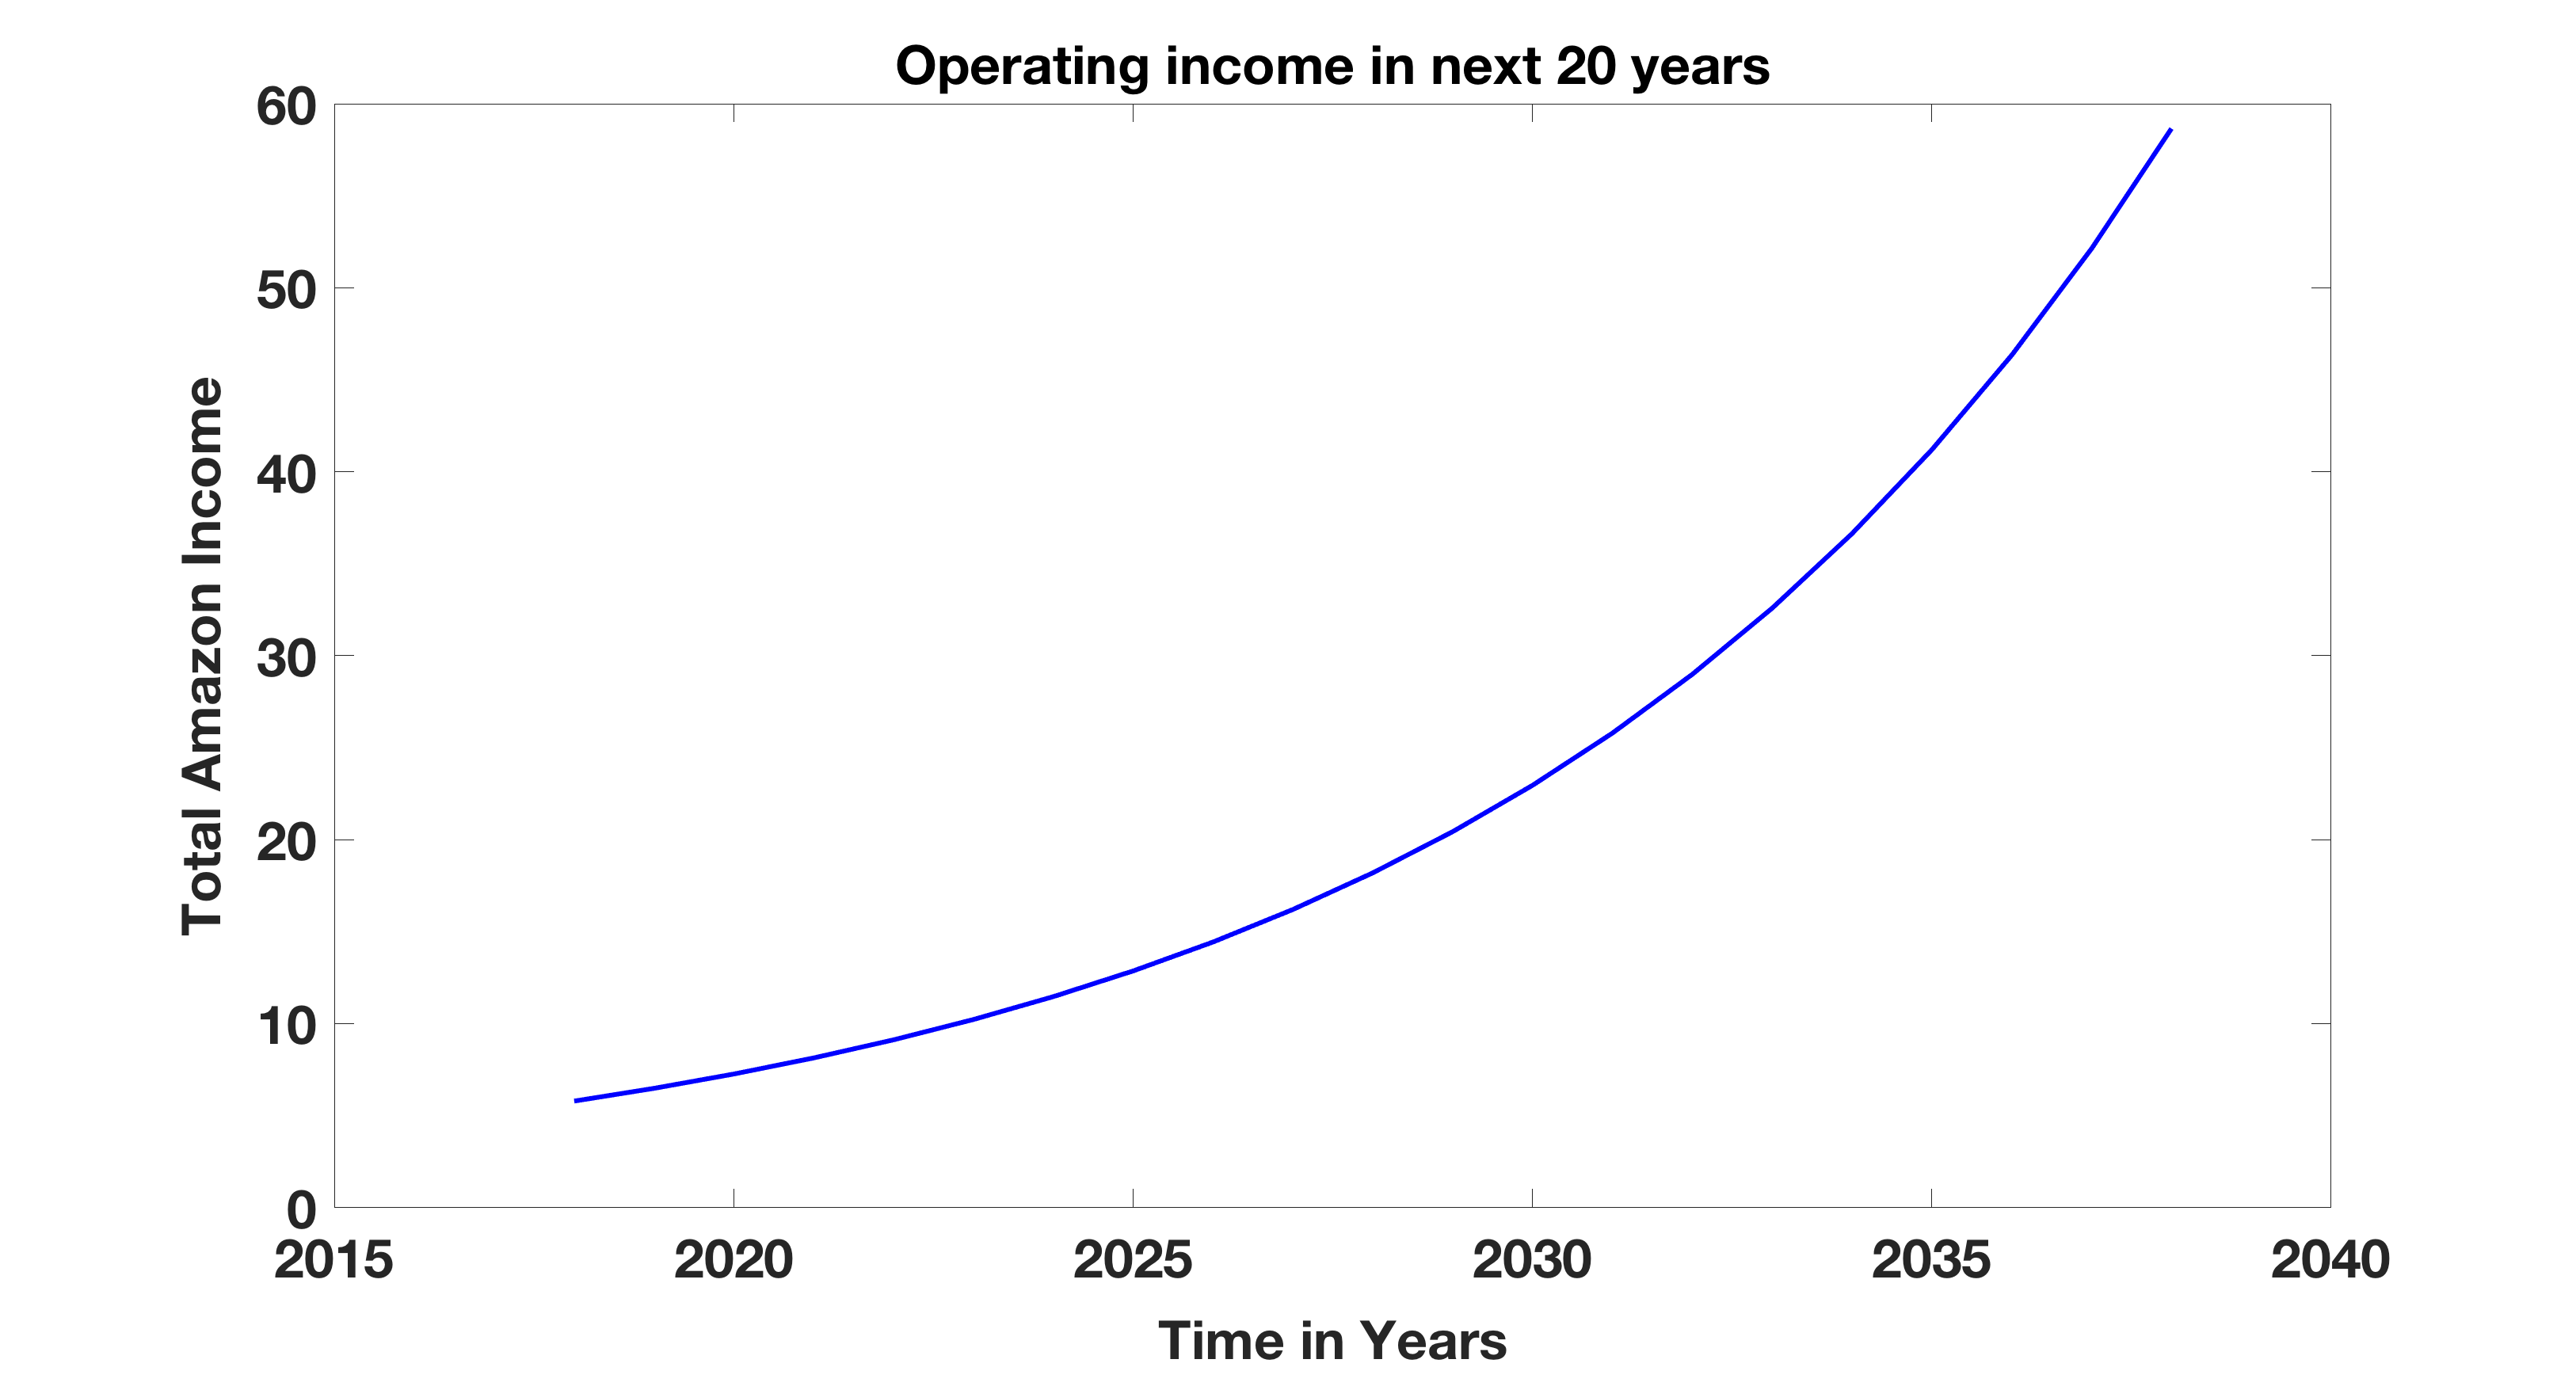
\includegraphics[width=\linewidth]{scen3income}
\caption{Operating income (USD, Billions) for next 20 years for Scenario \#3}
\label{fig:scen3income}
\end{figure}

The figure \ref{fig:scen3income} represents the operating income of Amazon for next 20 years. 

\textbf{Scenario \#4 - Amazon - A trillion dollar income company:}
In this scenario, the Amazon enterprise device a strategy where they grow aggressively in the AWS business segment with less impact to the existing customer and grow steadily in the Amazon North America business. In this scenario, few AWS customer may leave the AWS service and go to their competitor and since AWS will be growing aggressively, it will not have an impact.
\[
A =
\begin{bmatrix}
0.3 & -0.01 \\
-0.02 & 0.1
\end{bmatrix}
\]
\begin{figure}[ht]\centering
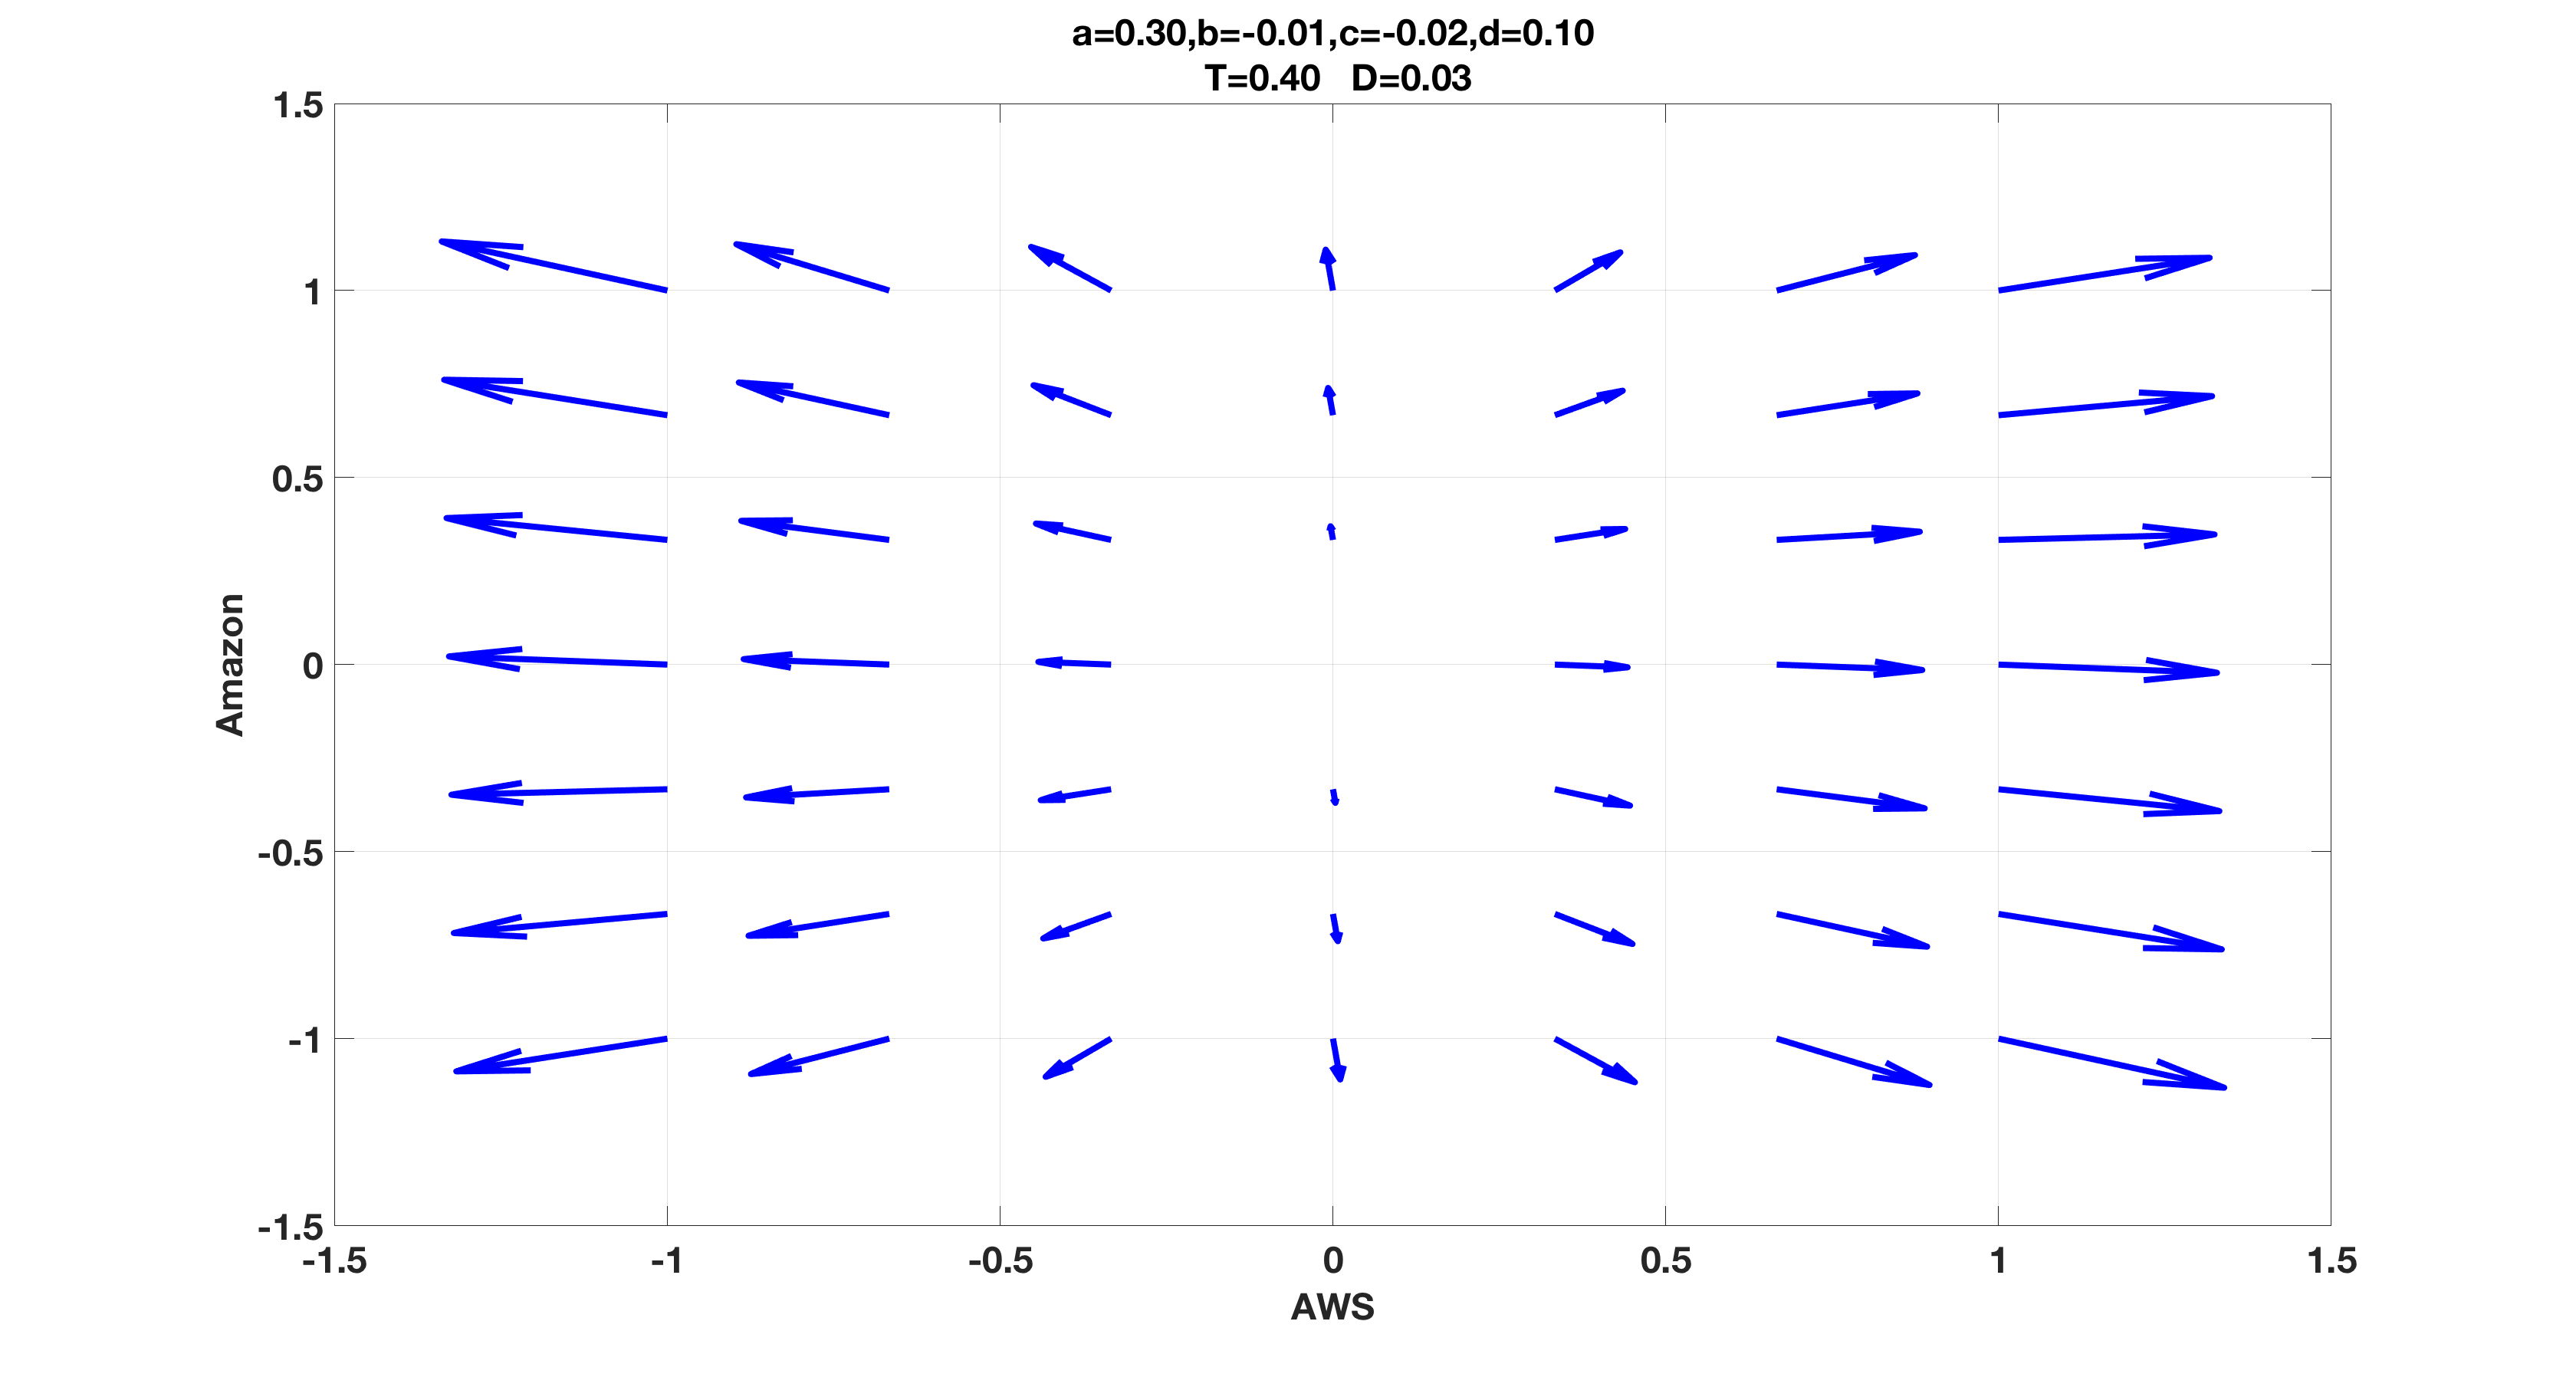
\includegraphics[width=\linewidth]{scen4}
\caption{Phase Portrait for Scenario \#4}
\label{fig:scen4}
\end{figure}  
Eigen values are $\lambda_1 = 0.3010$ and $\lambda_2 = 0.0990$ and Eigen vectors are given 
\[
V_1 =
\begin{bmatrix}
0.9951  \\
-0.0990 
\end{bmatrix}
,V_2 =
\begin{bmatrix}
0.0497  \\
0.9988
\end{bmatrix}
\]
$C_1=2.98$ and $C_2=2.65$.

The phase portrait is given in the figure \ref{fig:scen4} and implies that both the units exponentially grow in long term. 

\textbf{Long term Operating Income for Scenario \#4}
By using the framework established and the conditions set for this scenario based on $a$,$b$,$c$,$d$, the general operating income equation for Amazon (including the North America and AWS) are given below. 
\begin{equation} \centering
X(t) = 4.58^{0.12 t} + 1.19 e^{0.07 t}
\label{eq:s4}
\end{equation}

\begin{figure}[ht]\centering
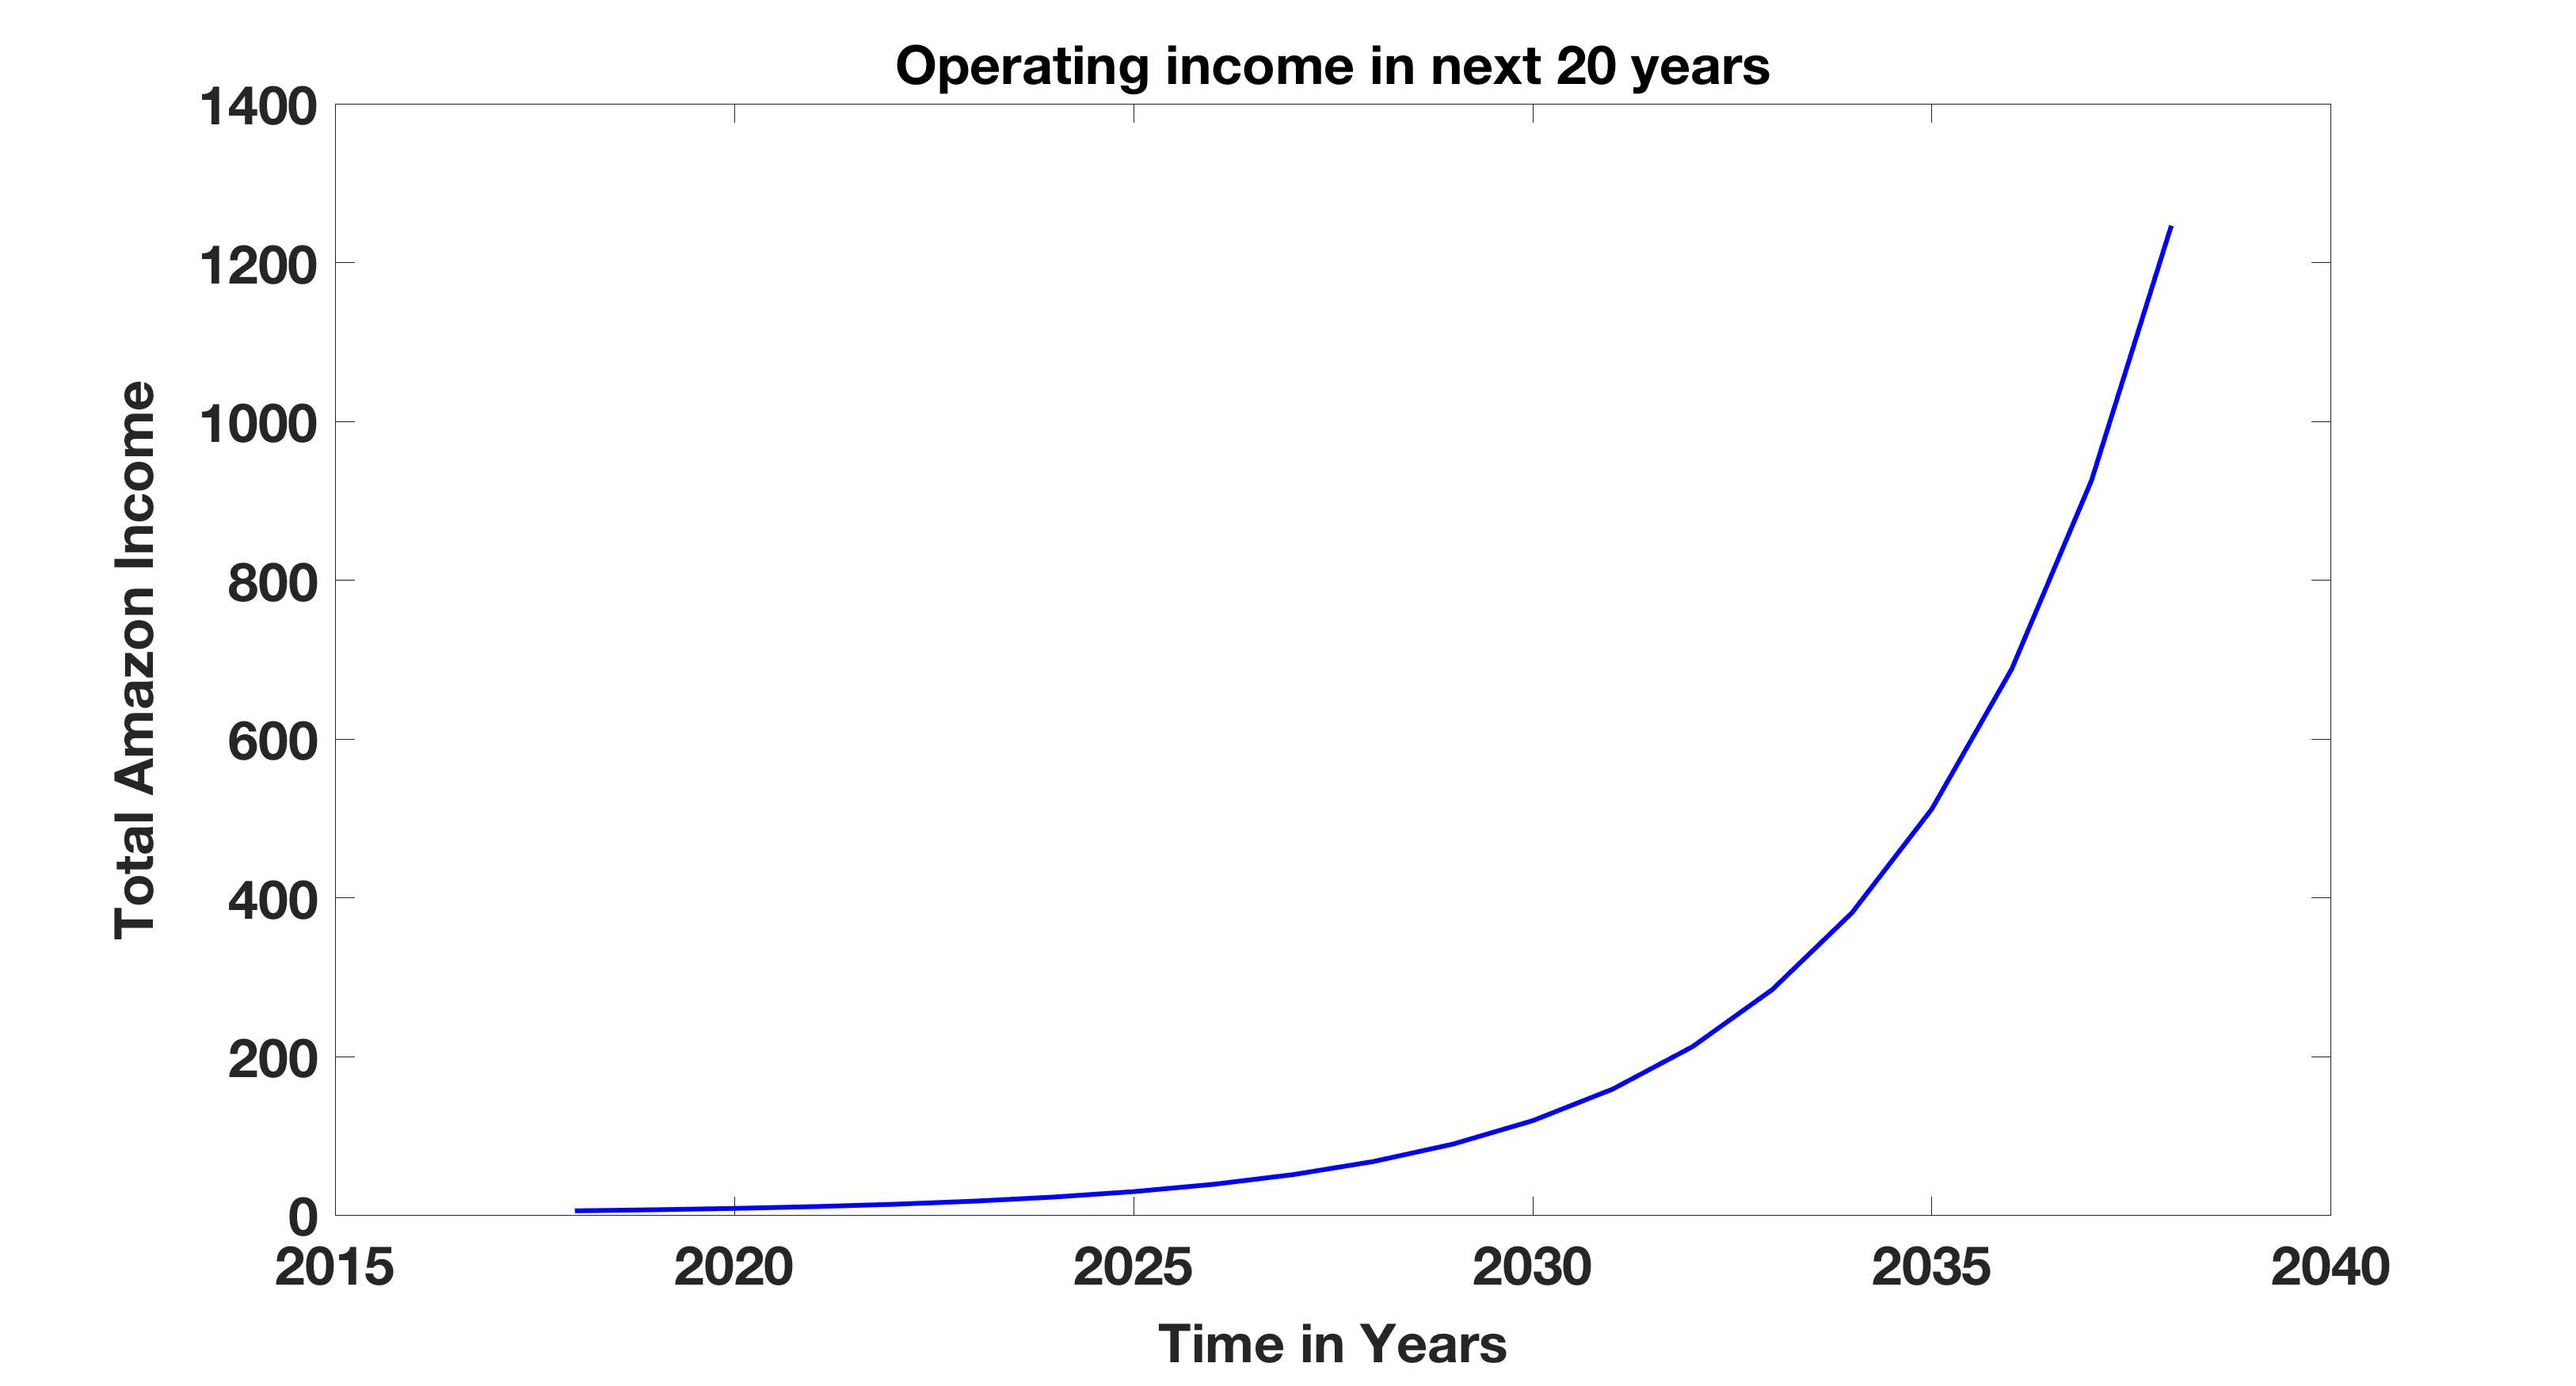
\includegraphics[width=\linewidth]{scen4income}
\caption{Operating income (USD, Billions) for next 20 years for Scenario \#4}
\label{fig:scen4income}
\end{figure}

The figure \ref{fig:scen4income} represents the operating income of Amazon for next 20 years. 

\subsubsection{Conclusion}
Scenario \#4 clearly indicates that if Amazon enterprise focuses on the cloud computing business, it will become a Trillion US dollars income company. As the expense ratio for the Amazon North America is relatively less comparing to the AWS and as per the initial survey, as of today, US market spends close to trillion dollars in the IT infrastructure, if Amazon focuses on the IT infrastructure ie. cloud computing business, within next 20 years, Amazon will become trillion income (not just revenue) company. However, there few scenarios (not shown in this paper), where the system has high sensitivity where Amazon become bankrupt in next 10 years as their competition from Microsoft and Google grows and they continue to build aggressive market disruptors willing to kill any established players like borders. 

This paper can be continued to study the dynamical system when Microsoft and Google become aggressive in their cloud computing business. 

%------------------------------------------------
\phantomsection
\section*{Acknowledgments} % The \section*{} command stops section numbering

\addcontentsline{toc}{section}{Acknowledgments} % Adds this section to the table of contents

Sincere appreciation to my loving wife Raji Praba and my loving kids Deepak Praba and Darshan Praba for their cooperation to work on this paper during the holiday (while watching Tamil Movies \& football)


%----------------------------------------------------------------------------------------
%	REFERENCE LIST
%----------------------------------------------------------------------------------------
\phantomsection
\bibliographystyle{unsrt}
\bibliography{sample}

%----------------------------------------------------------------------------------------

\end{document}
